% Created 2019-03-01 Fri 09:57
% Intended LaTeX compiler: pdflatex
\documentclass[11pt]{article}
\usepackage[utf8]{inputenc}
\usepackage[T1]{fontenc}
\usepackage{graphicx}
\usepackage{grffile}
\usepackage{longtable}
\usepackage{wrapfig}
\usepackage{rotating}
\usepackage[normalem]{ulem}
\usepackage{amsmath}
\usepackage{textcomp}
\usepackage{amssymb}
\usepackage{capt-of}
\usepackage{hyperref}
\usepackage{minted}
\usepackage[hyperref,x11names]{xcolor}
\usepackage{physics}
\usepackage{cases}
\graphicspath{ {./} }
\usepackage{tikz}
\usetikzlibrary{arrows,plotmarks,calc,positioning,fit}
\usetikzlibrary{shapes.geometric, decorations.pathmorphing, patterns, backgrounds}
\newcommand{\tikzremember}[1]{{  \tikz[remember picture,overlay]{\node (#1) at (0,11pt) { };}}}
\tikzset{snake it/.style={decorate, decoration=snake}}
\usepackage[nottoc]{tocbibind}
\author{Tigany Zarrouk}
\date{\today}
\title{Notes and Literature}
\hypersetup{
 pdfauthor={Tigany Zarrouk},
 pdftitle={Notes and Literature},
 pdfkeywords={},
 pdfsubject={},
 pdfcreator={Emacs 25.3.1 (Org mode 9.2.1)}, 
 pdflang={English}}
\begin{document}

\maketitle
\tableofcontents



\section{General notes}
\label{sec:org6fcaa11}

\subsection{Electronic Structure}
\label{sec:org2fd7e1c}
\subsubsection{Tight Binding}
\label{sec:org4de4e49}
\begin{enumerate}
\item Tight Binding Band Model
\label{sec:orgcbe6b80}

As with all tight-binding models, they are based on a linear combination of atomic orbitals basis. 
We compose our hamiltonian as a matrix that is in this basis, where each column/row corresponds to a particular
atom's orbital.
The \emph{on-site} terms are on the diagonal as these simply correspond to the energy of a particular orbital
e.g.\(\epsilon_s\), \(\epsilon_p\), \(\epsilon_d\), which are also parameters along with the assumed orbital occupancies 
of the free atoms \(N_{\mathbf{R}\ell}\).
The other terms are off diagonal terms which either represent the bonding between different atoms, if it is a matrix element
between two different atomic sites, or if the terms are on the the same atomic site, this represents an interaction
between orbitals on the same atom. These are crystal field terms and relate to the distortion of sperical symmetry arising from
interaction of orbitals on the same site, which causes a splitting of energy levels. 
In the tight binding model these come from the self-consistent polarisable tight-binding 
model. If the cutoffs between bond integrals is short, then the Hamiltonian matrix becomes sparse, 
which means that diagonalisation is quick. 

For the band model we have the density matrix composed in the normal way. 
$$ \hat{\rho} = \sum_{n} f_{n} \ket{n} \bra{n}$$ and it is straight forward to see that this density matrix satisfies 
$$ \hat{\rho} = N $$ where \(N\) is the number of electrons in this system. 

The band energy is then given by $$E_{\text{band}} = \text{Tr}\hat{\rho}\hat{H} = \sum_{n} f_{n}\epsilon_{n} $$, where \(\epsilon_{n}\)
is the energy of an eigenstate. This band energy is essentially the sum of the electron kinetic energies and electron-ion interaction energies. 

A pair potential is added to this to account for the electron-electron and ion-ion contributions to the total energy 
as given in density functional theory.
So the total energy is 

$$ E_{\text{tot}} =   E_{\text{band}} + E_{\text{rep}} $$


The band model is \emph{not} consistent with the force theorem, as the bond model is.
The force theorem states that there is no contribution to the force from self-consistent redistribution of charge 
as a result of the virtual displacement of an atom. 

There is no self-consistent charge redistribution in the band model.

If we move an atom in the band model, then there should be a change in the band structure energy from electron-electron interaction. 
However, all electron-electron interactions are controlled by the pair-potential, as per its definition so there is \emph{not} exact 
cancellation. 

This is exactly cancelled in DFT by the double counting term. 


\item Tight Binding Bond Model
\label{sec:org6c91632}

\begin{enumerate}
\item Paxton: Implementation by Diagonalisation.
\label{sec:orga9fcfa0}
This follows from \cite{Paxton:153084}

In the TBBM we use the \emph{covalent bond energy} as the fundamental quantity of interest that we want to calculate.
To obtain this energy, one simply ignores the diagonal terms when taking the trace over the product of the density matrix and
the Hamiltonian (when we calculate the band energy):)

\[ 
E_{\text{bond}} = \frac{1}{2} \sum_{\mathbf{R}L\mathbf{R}'L'//\mathbf{R}/neq\mathbf{R}'}
                             2\rho_{\mathbf{R}L\mathbf{R}'L'} H^{0}_{\mathbf{R}'L'\mathbf{R}L}.
\]


The terms we have excluded from the band energy are now grouped with the corresponding quantities in the free atom. 
This gives rise to the \emph{promotion energy}.

\begin{align}
E_{\text{prom}} &= \sum_{\mathbf{R}L} \Big(\rho_{\mathbf{R}L\mathbf{R}'L'}H^{0\mathbf{R}'L'\mathbf{R}L} - N_{\mathbf{R}\ell}\epsilon_{\mathbf{R}\ell} \Big)\\
              &= \sum_{\mathbf{R}L} \Big(\rho_{\mathbf{R}L\mathbf{R}'L'} - N_{\mathbf{R}\ell} \Big) \epsilon_{\mathbf{R}L}\\
              &= \sum_{\mathbf{R}L} \Delta q_{\mathbf{R}L} \epsilon_{\mathbf{R}\ell}
\end{align}

\begin{align}
E_{\text{prom}}^{\text{TBBM}} &= \sum_{\mathbf{R}L} \Big(\rho_{\mathbf{R}L\mathbf{R}'L'} - N_{\mathbf{R}\ell} \Big) H_{\mathbf{R}L\mathbf{R}L}\\
              &= \sum_{\mathbf{R}L} \Delta q_{\mathbf{R}L}( \epsilon_{\mathbf{R}\ell} + \Delta \epsilon_{\mathbf{R}\ell} )
\end{align}

Where the promotion energy represents the preparation of an atom going from the free state to that of one about to undergo bonding. 
E.g. the energy levels of particular atoms being prepared to undergo hybridisation.


The band model \emph{is} consistent with the force theorem as there is  self-consistent redistribution of charges. 
In the \emph{band} model there is no contribution to the forces from the promotion energy as 
\(\epsilon_{\mathbf{R}L}\delta q = \delta\epsilon{\mathbf{R}L} q = 0\) as the eigenvalues do not change: they are constants. 

However the Mulliken charge transfers are not necessarily zero, and the force theorem necessitates contributions due to  
electrostatic charge transfer to be included in the calculation of the interatomic force. This means that the band model is 
inconsistent due to its neglect of these terms. 

The self-consistency that is imposed in the TBBM bond model is that of \emph{local charge neutrality}. This means that the total charge 
on a particular site should equal that of the reference atom. This means that the \emph{total} Mulliken charge difference between that and
free atoms is \emph{zero}. 

This self consistency is achieved by adjusting the on-site orbital energies. This only affects the diagonal of the Hamiltonian 
so only \(E_{\text{prom}}\) changes. 

This means there is an additional contribtion to the force on atom \(\mathbf{R}\) which comes from \(\sum_{L} \Delta q_{L} \Delta \epsilon_{\ell}\). 

If all orbital energies are shifted by the same amount at each site, during self-consistency, then this term vanishes as 
\(\epsilon_{\ell}\) is independent of \$L\$---as \(L\) is the index which corresponds to angular momentum \(nlm\). 
So the term moves to the front of the summation, and as the sum of all changes in charges are zero, by local charge neutrality,
 then the term vanishes. 

\item Sutton 1988: The Tight-Binding Bond Model
\label{sec:org9a19d13}
\cite{Sutton1988}

\begin{enumerate}
\item General Formulation
\label{sec:orgd76b97e}
In the original paper of the tight-binding bond model, Sutton \emph{et al} obtain
the tight-binding bond model from the Harris-Foulkes functional.

If we say that the single particle potential of the Kohn-Sham equations is 
\begin{LaTeX}
\[
\widetilde{V}(\mathbf{r}) = v(\mathbf{r}) + V^{\text{f}}(\mathbf{r}) + \mu_{\text{xc}}(\mathbf{r})
\]
\end{LaTeX}

where 
\begin{itemize}
\item \(v(\mathbf{r})\) is the total ionic potential
\item \(V^{f}(\mathbf{r})\) is the Hartree potential (self-energy of the electron density.)
\item \(\mu_{xc}(\mathbf{r})\) is the exchange-correlation potential.
\end{itemize}

Then we can solve for the Hamiltonian once, and an output charge density \(\rho^{\text{out}}\) is
constructed from its eigenstates, without any self-consistency iterations.  

\begin{LaTeX}
\[
\widetilde{H} = -\frac{1}{2} \nabla^{2} + \widetilde{V}(\mathbf{r})
\]
\end{LaTeX}



The Harris-Foulkes functional, which exploits the variational principle, gives 
the leading corrections to the total energy are second order in the difference 
between \(\rho^{\text{f}}\), the input charge density and the exact charge density \(\rho^{\text{sc}}\). 

\begin{LaTeX}
\begin{align}
E = \sum_{n} f_{n} \tilde{\varepsilon_{n}} &- int \text{d}r \rho^{\text{f}}(\mathbf{r})
               \big( \frac{1}{2} V^{\text{f}}(\mathbf{r}) + \mu_{xc}^{\text{f}}(\mathbf{r})  \big)
               + E_{\text{xc}}[\rho^{\text{f}}] + E_{\text{ii}}\\
               &+ \mathcal{O}(\rho^{\text{sc}} - \rho^{\text{f}})^2 + \mathcal{O}(\rho^{\text{sc}} - \rho^{\text{out}})^2
\end{align}
\end{LaTeX}

where,
\begin{itemize}
\item \(\rho^{\text{f}}\) is an input charge density which is formed
from a superposition of isolated atomic charge densities. This if formed
from condensing atoms infinitely far apart without allowing the atomic
charge densities to change.

\item \(\rho^{\text{out}}\) is the charge
density formed from the \emph{eigenstates} of the Hamiltonian.

\item \(\rho^{\text{sc}}\) is the exact ground state charge density

\item \(f_{n}\) is the occupation number

\item \(\tilde{\varepsilon}_{n}\) is an eigenvalue of the single-particle
Hamiltonian.

\item \(E_{\text{ii}}\) is the ion-ion interaction energy.

\item \(\Delta E_{xc}[\rho^{\text{f}}]\)  which is the change in the exchange-correlation energy in forming the charge
density \(\rho^{\text{f}}\).
\end{itemize}

One obtains the binding energy as 
\begin{LaTeX}
\[
E_{B} = \text{Tr}( \rho^{\text{out}} - \rho^{\text{f}} )\widetilde{H} + \Delta E_{es}[\rho^{\text{f}}] + \Delta E_{xc}[\rho^{\text{f}}]
\]
\end{LaTeX}

Where 
\begin{itemize}
\item \(\rho^{\text{f}}\) is an input charge density which is formed
from a superposition of isolated atomic charge densities. This if formed
from condensing atoms infinitely far apart without allowing the atomic
charge densities to change.

\item \(\rho^{\text{out}}\) is the charge
density formed from the \emph{eigenstates} of the Hamiltonian.

\item \(\Delta E_{es}[\rho^{\text{f}}]\) is the change in electrostatic energy
of all valence electrons and ion cores when the atoms are condensed from
infinity to make the solid---which included electron-electron, electron-ion
and ion-ion electrostatic interactions

\item \(\Delta E_{xc}[\rho^{\text{f}}]\)  which is the change in the exchange-correlation energy in forming the charge
density \(\rho^{\text{f}}\).
\end{itemize}

They express \(\text{Tr}(\rho^{\text{out}} - \rho^{\text{f}})\widetilde{H}\) in the atomic
orbital representation as a sum over on-site terms and a sum over inter-site
terms. 




\begin{equation}
\text{Tr}(\rho^{\text{out}} - \rho^{\text{f}})\widetilde{H} =
   \underset{\text{Promotion Energy}}{ 
      \sum_{\substack{i \\ \alpha\beta}} 
         \big[ (\rho^{\text{out}})^{i\alpha i\beta} -
               (\rho^{\text{f}})^{i\alpha i\beta} \delta^{i\alpha}_{i\beta} \big]
         \widetilde{H}_{i\beta i\alpha} 
            }
  + \underset{\text{Covalent Bond Energy}}{
      \underset{i \neq j}{ \sum_{i \alpha}\sum_{j \beta} }
         (\rho^{\text{out}})^{i\alpha i\beta} \widetilde{H}_{j\beta i\alpha}
                }
\end{equation}

In ther first term, in a perfect cubic crystal, 
\(\widetilde{H}_{i\alpha i\beta} = \widetilde{H}_{i\alpha i\beta}
\delta^{i\beta}_{i\alpha}\).
The diagonal elements \(\widetilde{H}_{i\alpha i\alpha}\) are the free atomic
term values corrected by the crystal-field terms in the solid. So this first
term is the promotion energy: the enrgy associated with the change of
occupancy of the atomic orbitals on forming the solid from free atoms. 

if the atomic environment around each site in the solid is distorted then
\(\widetilde{H}_{i\alpha i\beta}\) are non-zero because of crystal-field terms.

It is possible to disgonalise the part of the Hamiltonian \(\widetilde{H}\)
associated only with site \(i\) and thys express the terms involving site \(i\) in
this equation, but the new diagonal elements of \(\widetilde{H}\) will vary from site
to site.

The second term is the covalent bond energy of the solid and it si equal to
the sum of the covalent energies of individual bonds between orbitals on
different atoms. This bond energy is part of the band energy of the solid

\begin{LaTeX}
\begin{align}
E_{\text{cov}} &= \frac{1}{2}  \underset{i \neq j}{ \sum_{i \alpha}\sum_{j \beta} }
         (2 \rho^{\text{out}})^{i\alpha i\beta} \widetilde{H}_{j\beta i\alpha}\\
               &= E_{\text{band}} - 
              \sum_{\substack{ i\\ \alpha\beta}} 
                   (\rho^{\text{out}})^{i\alpha i\beta}
                    \widetilde{H}_{j\beta i\alpha}
\end{align}
\end{LaTeX}


They further argued that the terms \(\Delta E_{xc}[\rho^{\text{f}}]\) 
\(\Delta E_{es}[\rho^{\text{f}}]\) can be approximated by a repulsive pair potential
centred at atomic sites.

So then the binding energy can then be expressed as a sum of bond energies and
promotion energies, where each bond energy is a sum of the covalent energy of
the bond and the pair potential interaction. 

\item Interatomic forces
\label{sec:org16bdedc}

The forces on each atom can be found by differentiating the binding energy
with respect to \(\mathbf{r}\), using the relation between the density matrix
and the Green's function,
\[
(\rho^{\text{out}})^{i\alpha i\beta} = -\frac{2}{\pi} \Im \int^{E_{\text{F}}} 
   G^{i\alpha j\beta} (E^{+}) \text{d}E
\]
and 
\[
 -\frac{1}{\pi} \Im \sum_{i \alpha} H_{p\mu i\alpha} G^{i\alpha l\gamma}
     =  -\frac{1}{\pi} \Im E G_{p\mu}^{l\gamma}
\]
with the Hellmann-Feynman theorem, which has also been derived by
\cite{Foulkes1989}. 

So the derivative of the binding energy with respect to \(x_k\) is 

\begin{equation}
\frac{\partial E_{\text{B}}}{\partial x_{k}} = 
   \frac{1}{2}\sum_{i\alpha}\sum_{j\beta} 2(\rho^{\text{out}})^{i\alpha}_{j\beta}
       \frac{\partial H^{j\beta}_{i\alpha}}{\partial x_{k}}
 - \sum_{i\alpha} (\rho^{\text{f}})^{i\alpha i\alpha} 
                  \frac{\partial H_{i\alpha i\alpha}}{\partial x_{k}}
 + \frac{\partial}{\partial x_{k}} \big(\Delta E_{xc}[\rho^{\text{f}}] + \Delta E_{es}[\rho^{\text{f}}] \big )
\end{equation}


This can be simplified with the following approximations:

\begin{enumerate}
\item The non-orthogonality of the atomic-orbital basis set may often be
neglected becasue the leading correction terms to the energy are \emph{second
order} in the overlap matrix.
\item Three-centre terms may be neglected because the leading three-centre
corrections to the energy are also of second order.
\item Assume that 
\(\widetilde{H}_{i\alpha i\beta} = \widetilde{H}_{i\alpha i\alpha}
   \delta^{i\beta}_{i\alpha}\) i.e. the Hamiltoniam matrix elements between
\emph{different orbitals} on the same atom may be neglected.
\item Each atom may be assumed to remain charge neutral by varying the on-site
Hamiltonian matrix elements in such a way that the energy splitting
between different orbitals on the same atom are preserved.
\begin{itemize}
\item This approximation ensures that contributions to the force in the above
equation from on-site terms in ther first sum cancel those of the second sum
\item This leads to consistency with the force theorem.
\end{itemize}
\end{enumerate}

These approximations give the derivative of the binding energy to be:

\begin{equation}
\frac{\partial E_{\text{B}}}{\partial x_{k}} = 
   \sum_{j \neq k}\sum_{\alpha\beta} 2(\rho^{\text{out}})_{k\alpha j\beta}
       \frac{\partial H_{j\beta k\alpha}}{\partial x_{k}}
  + \frac{\partial}{\partial x_{k}} \big(\Delta E_{xc}[\rho^{\text{f}}] + \Delta E_{es}[\rho^{\text{f}}] \big )
\end{equation}

\item Local Charge Neutrality
\label{sec:org870478c}

The approximation to local charge neutrality is motivated by 
\begin{enumerate}
\item In a metal where there is perfect screening any excess charge associated
with an atom will be neutralised---similarly in a semiconductor where the
band gap is much smaller than the widths of the valence and conduction
bands the screening length is approximately the same as an inter-atomic
separation and hence local charge neutrality will be a good
approximation.
\item To obtain the correct bulk modulus of the solid when it is calculated by
the method of long waves or by homogeneous dilatation, the charge density
must be treated within a self-consistent scheme, and LCN is the simplest
assumption to make.
\item There would be long range Coulomb terms if local charge neutrality were
not required, in binary systems. Is is always possible to find a basis
where each atom is neutral.
\item Charge neutrality within the TBBM leads to an internally consistent
picture of the heats of formation of transition metal alloys.
\end{enumerate}

This local charge neutrality is achieved by varying the on-site terms of the
Hamiltonian matrix elements. In general there would be contributions from the
intersite Hamiltonian matrix elements as the electronic charge is distributed
throughout the system. 

The explicit dependence of on-site Hamiltonian matrix elements on the
positions of neighbouring atoms appears in the model in the pair potential
because the on-site crystal-field terms contribute for example to \(\Delta
E_{es}\). So the requirement for local charge neutrality results in the
on-site Hamiltonian matrix elements depending on the positions of neighbourigh
non-equivalent atoms. 

The energy splittings betweem orbitals are assumed to be constant at each
atomic site so all the diagonal Hamiltonian elements change by the same amount
\(\delta \widetilde{H}_{i}\). This means ther eare no contributions to the force
from the promotion energy as discussed before. 

The bond order is determined by all inter-site and on-site Hamiltonian matrix
elements in the local atomic environment. So the forces from the covalent bond
terms are not simply two-body interactions even though the total force cay be
expressed as a sum of forces from each neighbouring atom. 

Self-consistency is important when it comes to calculating force
constants. With homogeneous strain all monatomic basis atoms remain equivalent
and therefore there is no charge transfer. 
However, if there is a volume change with the strain (NOTE: does this mean
that you can have a compression and tension, which conserves volume, in this
sense?), the Fermi level changes
and this gives rise to an important change in the energy which is second order
in the strain \cite{Heine1980}. 

\begin{enumerate}
\item Priester Ge-GaAs Justification
\label{sec:orgbe458a3}
From \cite{Priester1986} local charge neutrality was motivated in a Ge-GaAs
interface. 

All inter-atomic matrix are specified and the intra-atomic (on-site) terms are
adjusted to within an additive constant. These on-site terms become very
important when it comes to dealing with interfaces. 

\[
\Delta = \bar{ E }( \text{ GaAs } ) - \bar{ E }( \text{ Ge } )
\]

where \(\bar{ E }( \text{ GaAs } )\), \(\bar{ E }( \text{ Ge } )\) are average \(sp^3\) energies 
(in the compound \(\bar{E}\) is the average between the Ga and As \(sp^3\)
energies). These are the on-site terms. 

The charge disturbance is near the vicinity of the interface and it has been
shown that the screening length roughly \(\sim 2\AA\), on the order of the
interplanar spacing. So one finds bulk values away from the interface. 

One wants to find this \(\Delta\) so the valence-band maxima in each material
are positioned with respect to each other to obtain a band offset. 

There is only electron transfer between the two
interface planes. As there are two atoms per two-dimensional unit cell, the
electron transfer can be split into two components \(\delta N_1\) from Ga to Ge
and \(\delta N_2\) from As to Ge, where the difference is from the population of
the state compared to that of the bulk, which is the change in electron
concentration due to the formation of the interface. 

If all on-site terms of an atom \(i\) are shifted by the same
amount \(U_{i}\), from the reference state, then we can express this as a sum
over excess populations on each other atom
\[
U_{i} = \sum_{j} \gamma_{ij} \delta N_{j}
\] 
where \(\gamma_{ij}\) are the corresponding intra- and inter-atomic Coulomb
terms. 

One can express \(\delta N_{i}\) in terms of the \(\delta N_{i}^0\) of the
reference situation so, when linearized

\[
\delta N_{i} = \delta N_{i}^0 + \sum_{j} X_{ij}U_j
\]

Solving in matrix form gives 

\[
U = ( 1 - \gamma X)^{-1} \gamma \delta N^0
\]

where \(X\) is the susceptibility matrix. If the eigenvalues of the matrix
\(\gamma X\) are much larger than 1 then we have approximate solutions 

\[
U \approx - X^{-1} \delta N^0
\]

which is exactly the result that one would obtain by local charge neutrality:
\(\delta N = 0\).

The important point is that in the reference situation, where all intra-atomic (on-site)
terms take their bulk values and \(\Delta = 0\), the quantities \(\delta N_1\),
\(\delta N_2\) do not exactly compensate. 

This means that there is a dipole layer with an average excess population of
\(( \delta N_1 + \delta N_1)/2\) per atom in the Ge plane. The effect of this
dipole layer is to shife the average \(sp^3\) level on one site with respect to
the other, i.e. to make the quantity \(\Delta \neq = 0\). 

So local charge neutrality tells us that 


$$\delta N_1(\Delta) + \delta N_2(\Delta) = 0$$
\end{enumerate}
\end{enumerate}
\end{enumerate}

\item Self-Consistent Polarisable-Ion Tight-Binding
\label{sec:org9e3ee97}
Following \cite{Paxton:153084}. Original paper by \cite{Finnis1997}.


Remember that the expansion of the Hohenburg-Kohn-Sham functional to second order in the energy, if \(H = H^0 + H'\),
where \(H^0\) is the Hamiltonian generated from the reference charge density \(\rho^0\) (about which the HKS functional has been expanded)


\begin{align}
E^{(2)} = &\sum_{n} f_{n} \bra{n} H^{0} \ket{n} %\expval{H^{0}}{n} \\
&- \int \rho^{0}(\mathbf{r}) V^{0}_{xc} \text{d}\mathbf{r} - E_{H} + E^{0}_{xc} + E_{ZZ}\\
&+ \frac{1}{2} \int \text{d}\mathbf{r} \int \text{d}\mathbf{r}' \Big{ 
 e^2 \frac{\delta\rho(\mathbf{r})\delta\rho(\mathbf{r}')}{|\mathbf{r} - \mathbf{r}'|} \Big} \\
& \delta\rho(\mathbf{r})\frac{\delta^2E_{xc}}{\delta\rho(\mathbf{r})\delta\rho(\mathbf{r}')}\delta\rho(\mathbf{r}')
\end{align}

Where the first two lines are the \emph{Harris-Foulkes Functional}.

This is because, as a potential changes, 

In terms of multipole moments, we cannot construct these from the charge density as we do not calculate one. 
We can however use the eigenvalues such that we can construct them. 

So we can construct the multipoles in terms of the expansion coefficients. 



\begin{equation}
Q_{\mathbf{R}L} = \sum_{L'L} \sum_{n}  f_{n} \bar{c}_{\mathbf{R}L}^{n} c_{\mathbf{R}L}^{n} 
                        \bra{\mathbf{R}L'}\hat{Q}_{\mathbf{R}L}\ket{\mathbf{R}L''}
\end{equation}


\item Trinkle 2006
\label{sec:orgc060de5}
\begin{itemize}
\item Collapse problem found in tight binding if atoms come too close
together. Electrons go in the bonding state and not the anti-bonding
state and so the energy goes down
\item Can be fixed by implementing spline potential that levels off below a
given cutoff, which effectively simulates a pair potential.
\item Environmentally dependent on-site terms were used instead of a pair potential.
\item These on-site energies are dependent on the local density \(\rho_{i}\) and
they have a cutoff function \(f_{c}(r_{ij})\) which has fixed parameters
\(R_{0}\) and \(l_{0}\).\#+BEGIN\textsubscript{EXPORT} latex
\end{itemize}
\begin{equation}
      \epsilon_{i,l} = a_{l} + b_{l}\rho_{i}^{2/3} + c_{l}\rho_{i}^{4/3} +
      d_{l}\rho_{i}^{2}\end{equation}
\#+END\textsubscript{EXPORT} 
      \[ \rho_{i} = \sum_{j \neq i} \text{exp}\big\{ -\lambda^{2} r_{ij}
      f_{c}(r_{ij}) \big\} \]
      \[ f_{c}(r) = \frac{1}{1 + \text{exp}\Big\{  \frac{r-R_{0}}{l_{0}}\Big\}
      }\]

\item Notation
\label{sec:org7c1e5b5}

Some nice tensor notation was introduced by \cite{Ballentine1986}

This has a nice correspondence between the metric tensor in General Relativity
and the overlap matrix \(S_{\alpha\beta}\), where it raises and lowers indices
of vectors etc.
\end{enumerate}

\subsubsection{DFT}
\label{sec:orgb192204}
\begin{enumerate}
\item Hartree-Fock
\label{sec:orgcd10164}
\begin{itemize}
\item Hartree-Fock is a method of calculating the energy of a configuration
with exact exchange.
\item This is done by essentially putting everything we don't know into the
kinetic energy functional.
\item Hamiltonian is split into contributions:
\begin{itemize}
\item \[\hat{H} = \hat{T} + \hat{V}_{ \text{ext} } + \hat{G}\]
\item \(\hat{G} = \hat{J} - \hat{K}\)
\item \(\hat{J}\) is the coulombic interaction:
\item \[ \bra{ \mathbf{r} } \hat{J} \ket{ \mathbf{n} } = \int \frac{ \bra{\mathbf{r}}\ket{n} }{|\mathbf{r} - \mathbf{r'}  |}d\mathbf{r} \]
\item So \[ E_{\text{H}} = \int \frac{\rho{\mathbf{r}\rho{\mathbf{r}'}}}{|\mathbf{r} - \mathbf{r'}|}\]
\item This includes fictitious self-interaction of electron density.
\item The Exchange functional removes this part, thus lowering the energy
\end{itemize}

\item This method is used in Hybrid DFT. This corrects band gaps mainly. But
there are also problems.
\end{itemize}

\item Functionals
\label{sec:orgb5f9884}
\item LMTO
\label{sec:org101e91c}
\end{enumerate}

\subsubsection{LMTO Suite}
\label{sec:org229dd71}
\begin{enumerate}
\item TBE Pair potentials and Bond integrals
\label{sec:orgf59cd21}
\begin{enumerate}
\item Pair potentials in tbe code
\label{sec:orga691250}
\begin{itemize}
\item Pair potential is constructed by \href{file:///home/tigany/lm/tb/makvpp.f}{makvpp.f}.
\item This calls \href{file:///home/tigany/lm/tb/vppder.f}{vppder.f} which actually evaluates the pair potential at that
point
\item In makvpp.f, if in the range of \(r_1 < r < r_{\text{c}}\), then
augmentative/multiplicative polynomial is used.
\begin{itemize}
\item To make this polynomial \href{file:///home/tigany/lm/tb/pcut45.f}{pcut45.f} is used.
\item Depending on the degree of polynomial we have this structure:
\begin{minted}[]{fortran}
      rr = r1 - r2
      xr1 = x - r1
      xr2 = x - r2

      c = val*rr*rr
      if (n == 5) then
	pnorm = rr**(-5)
	a = (0.5d0*curv*rr - 3d0*slo)*rr + 6d0*val
	b = (slo*rr - 3d0*val)*rr
      elseif (n == 4) then
	pnorm = rr**(-4)
	a = (0.5d0*curv*rr - 2d0*slo)*rr + 3d0*val
	b = (slo*rr - 2d0*val)*rr
      p2 = pnorm*(c + xr1*(b + xr1*a))
      dp2 = pnorm*(b + xr1*2d0*a)
      ddp2 = pnorm*2d0*a
      e = p2 * xr2**(n-2)
      de = (xr2*dp2 + float(n-2)*p2) * xr2**(n-3)
      dde = (xr2*xr2*ddp2+float(2*(n-2))*xr2*dp2+float((n-2)*(n-3))*p2)
C ... e, de and dde are the values and derivatives of the polynomial in the region r1 , r < rc
\end{minted}
\item So the form of the polynomial used is
\begin{itemize}
\item $$ P_5(x) = (x-r_2)^3 P_2(x)  $$
\item \[ P_2(x) = a(x-r1)^2 + b(x-r_1) + c \]
\item \[ a = \frac{1}{ (r1-r2)^5 } \big\{  \frac{1}{2}(r_1-r_2)^2f"(r_1) -3(r_1-r_2)f'(r_1) + 6f(r_1) \big\} \]
\item \[  b = \frac{1}{(r_1-r_2)^4} \big\{ f'(r_1)*(r_1-r_2) - 3f(r_1) \big\}  \]
\item \[ \frac{1}{(r_1 - r_2)^5} x \]
\item \[  c = \frac{ f(r_1) }{ (r_1-r_2)^3} \]
\item Where \(f(x)\) is the function that needs to be cut
\end{itemize}
\end{itemize}
\item Current model has this
\begin{minted}[]{bash}
Ti,Ti:
   type 2 (Exp. decay), V(d) = a exp (- b d)
	     dds    ddp    ddd
   coeff:  -2.75   1.84  -0.46
   decay:   0.71   0.71   0.71
   cutoff type 2 (multiplicative), 5th order polynomial, range [r1, rc]
	     dds    ddp    ddd
   r1:      6.20   6.20   6.20
   rc:      8.50   8.50   8.50

\end{minted}
\end{itemize}



\item Bond integrals from tbe
\label{sec:org69e91a3}
\begin{itemize}
\item So bond integrals from titanium look like this, from this file
\href{file:///home/tigany/Documents/ti/complete\_titanium/ti\_01-11-18/plot\_bond\_integrals/plot\_bond\_integrals.py}{plot\textsubscript{bond}\textsubscript{integrals.py}}
\end{itemize}
\begin{figure}[htbp]
\centering
\includegraphics[width=.9\linewidth]{/home/tigany/Documents/ti/complete_titanium/ti_01-11-18/plot_bond_integrals/tbe_bond_integrals_with_polynomial_cutoffs_multiplicative_alt.png}
\caption{\label{fig:org2c5c260}
Bond integrals with multiplicative polynomial cutoffs.}
\end{figure}
\begin{figure}[htbp]
\centering
\includegraphics[width=.9\linewidth]{/home/tigany/Documents/ti/complete_titanium/ti_01-11-18/plot_bond_integrals/tbe_bond_integrals_with_polynomial_cutoffs_multiplicative_zoomed_in.png}
\caption{\label{fig:orgdea6679}
Bond integrals with multiplicative polynomial cutoffs: zoomed in.}
\end{figure}

\item Bond Integrals for first neighbour interaction
\label{sec:orge6456a3}
To make first neighbours it is optimal to have a cutoff that is within
alat and \$1.4 \texttimes{} \$ alat. This is within the next shell of 6 neighbours
and so having the cutoff between alat and \(1.2\times\) alat should be
optimal. 
\begin{figure}[htbp]
\centering
\includegraphics[width=.9\linewidth]{/home/tigany/Documents/ti/complete_titanium/ti_01-11-18/plot_bond_integrals/check_new_cutoffs/cutoffs_at_alat_and_one_point_four_alat.png}
\caption{\label{fig:org81d2df1}
Bond integrals with multiplicative polynomial cutoffs for first neighbour interactions: zoomed in.}
\end{figure}
\end{enumerate}

\item Running lmf
\label{sec:orgaed2496}
\begin{enumerate}
\item Run Generic Calculation
\label{sec:org213f07d}
Run:
\begin{itemize}
\item lmchk --getwsr ti
\item Copy the old rmax into the R category in SPEC
\item lmfa ti -vhcp=1
\item Copy basp0 to basp
\item Run lmf
\end{itemize}
\end{enumerate}
\end{enumerate}

\subsubsection{BOP}
\label{sec:org3f74788}
\begin{enumerate}
\item Stefan Znam 2001 Thesis
\label{sec:org8bd8fa1}
\begin{enumerate}
\item Cauchy Pressures
\label{sec:orge3c6560}
\begin{itemize}
\item Cauchy pressures have zero contribution from pair potentials at
equilibrium.
\item Generally all Cauchy pressures in many-body central force models,
describing atoms embedded in an electron gas of the surrounding
neighbours, are positive when experimentally they are negative.
\begin{itemize}
\item This is the case with EAM and Finnis-Sinclair models.
\end{itemize}
\item In TiAl the environmental screening effects are most profound in the
case of s and p orbital overlap repulsion, as these orbitals are being
squeezed into the core region under the influence of unsaturated
covalent d bonds.
\end{itemize}
\begin{enumerate}
\item Reason for Cauchy Pressures
\label{sec:org248ee23}
\begin{itemize}
\item The reason for negative Cauchy pressures is meant to be from covalent
character of d bonding, but when using tight binding models, which
account for this, the cauchy pressure issue is not resolved.
\item These effects are explained in detail with regards to tight binding in
Nguyen-Manh, Pettifor, Znam, Vitek: Negative Cauchy Pressure Within
The Tight-Binding Approximation.
\item This warrants the need for environmental terms:
\begin{itemize}
\item The physical reasoning behind these terms are due to the repulsion
between orbitals in the atom.
\end{itemize}
\end{itemize}
\item Why TB can't have negative Cauchy Pressures
\label{sec:org8d895b0}
\begin{itemize}
\item TB only has contributions from the bond part of the interactions as the
pair potential at equilibrium has no contribution to the Cauchy
Pressures.
\item Failure of TB to reproduce negative Cauchy pressures because the
orbitals are tightly bound: interactions extend out only to nearest
neighbour atoms.
\item This requires that orbitals are not \emph{unscreened} atomic
orbitals.
\item Orbitals must be screened.
\item For transition metals, the valence d orbitals aren't screened as they are
tightly bound anyway.
\end{itemize}
\item Thoughts: What does this mean for Tight Binding
\label{sec:orgf2f4042}
\begin{itemize}
\item As the Cauchy pressure contributions only come from the bond integrals
and the pair potential, then the reason that some of the Cauchy
pressures are off are because these terms might not be necessarily
correct.
\item There are screening of these bond integrals, hence the Yukawa terms,
which change the interaction of these bond integrals.
\item These classical environmental terms modify the elastic constants by
including physically motivated screening terms in terms in terms of
Ti-Al as there is some repulsion from s-p overlap, as these orbitals
are squeezed into the core from the unsaturated d bonds.
\item These \emph{reduce} the Cauchy pressures such that they are negative
()
\end{itemize}
\end{enumerate}
\end{enumerate}
\item Environmental terms
\label{sec:org9ba9849}
\cite{NguyenManh2000}

Analytic environment dependent terms for tight-binding bond integrals were
formulated by Nguyen-Manh. One can express a non-orthogonal tight binding
model in terms of these environmental terms. 

Orthogonal TB models which are robust and transferable require the two-center
TB parameters to be environmentally dependent. 

Environmental terms take the form of a \emph{screening} function \(S^{ij}_{ll'\tau}\),
which is a hyperbolic tangent with argument 

\begin{equation}
\xi^{ij}_{ll'\tau} = A_{ll'\tau} \sum_{k \neq i,j} exp \Big[
    - \lambda_{ll'\tau} \Big( 
              \frac{R_{ik} + R_{kj}}{R_{ij}} \Big)^{\eta_{ll'\tau}} \Big],
\end{equation}

with \(l\), \(l' = s\), \(p\) or \(d\) and \(\tau = \sigma\), \(\pi\) or \(\delta\), with
\(A\), \(\lambda\) and \(\eta\) as fitting parameters. 

So that the bond integrals between a pari of atoms \(i\) and \(j\) takes the form 

\[
\widetilde{\beta}^{ji}_{ll'\tau} = \beta_{ll'\tau}(\kappa R_{ij}) ( 1 - S^{ij}_{ll'\tau}).
\]

Starting from the \emph{non-orthogonal} two-center TB approximation 
\[
( H - \epsilon_{n} S  )c_{n} = 0,
\]
where this \(S = \bra{i\mu lm}\ket{j\nu l'm'} = I + O\) is the nonorthogonality matrix with \(O\) being the
overlap matrix. The orbitals \(\ket{i\mu l}\) can be thought of already being
normalised by their local atomic environment. 

We can have an \emph{orthogonal} two-center TB secular equation of the form 

\[
(S^{-1}H - \epsilon_{n}I)c_{n} = 0
\]
but \(S^{-1}H\) is not Hermitian and it can be expressed as the sum of
antisymmetric and symmetric terms, as it is a real matrix:

\[
S^{-1}H = \frac{1}{2} ( S^{-1}H + HS^{-1}) + \frac{1}{2}( S^{-1}H - HS^{-1})
\]

The antisymmetric contribution vanishes if, say for \$s\$-valent systems, we have the
Wolfsberg-Helmholtz approximation \(\beta_{ss\sigma} = -AS_{ss\sigma}\) and the
approximation that all sites have the same on-site energy. 
\emph{This is assumed to be generally true}.


Elements of \(S^{-1} =  (I + O)^{-1}\) can be obtained from their BOP. Which
expresses the elements of the Green's function matrix \(G(E) = (EI - H)^{-1}\)
in a rapidly convergent real-space manner by imposing the physical constraint
that at any level of approximation the poles of the intersite Green's function
G\textsubscript{ij} are the same as those of the averate on-site Green's function
\$(1/2)(G\textsubscript{ii} + G\textsubscript{jj}). 


Going to \emph{three} recursion levels in BOP is exact for the inversion of
\(3\times 3\) matrices as would be relevand fro a three-atom s-valent trimer. 

The corresponding L$\backslash$:owdin expansion would hve replaced a determinant by unity
which is a poor approximation as the overlap integrals are not small. 

The central result is then 

\begin{equation}
S^{ij}_{ll'\tau} = \frac{ (c^{ij})_{ll'\tau} - (\bar{\mu}_2)_{ll'\tau} +
         (\bar{\mu}_{3})_{ll'\tau} }{ 1 +  O^2_{ll'\tau}(R_{ij})  - 2(\bar{\mu}_2)_{ll'\tau} +
                               (\bar{\mu}_{3})_{ll'\tau} }
\end{equation}

where the average \$p\$th moment is
\(\bar{\mu}_p = (1/2)(\mu^i_p + \mu^j_p)\).

The calculation asumes that the screening of the \(ij\) bonds is carried out bia
the valence \(s\) orbitals on the neighbouring sites \(k\). 

Valence \(p\) and \(d\) contributions to the screening are much
weaker. All four-body contributions were neglected and the off-diagonal
elements are the same as that of the \(ij\) bond of whose screening is of
interest. 

There is a large discontinuit between first and secon neighbours for the
\(dd\pi\) and \(dd\delta\) bond integrals but the \(dd\sigma\) bond integrals are
continuous. This is because the angular dependence of the screening function
vanishes which leaves the \(dd\sigma\) bond integral unscreened (due to the bond
angle in bcc). 

On the other hand the \(dd\pi\) integral is heavily screened with
the slope and magnitude being reduced by a factor of 3. This is critical when
it comes to the behaviour of second-neighbour force constants and removes the
problem of the unstable T2 phonon mode at the N point that is found in most
two-center TB fits. 
\item Finite Electron Temperature
\label{sec:orgdbdee45}
\begin{enumerate}
\item Gillian 1986
\label{sec:org3dcd0cb}
\cite{Gillan1989}

Finite electron temperature for estimation of the band energy at zero kelvin. 

The finite-temperature scheme is merely a device, whose main purpose is to
smooth discontinuities at the Fermi level.

Really want to get the ground state energy \(E_0\), for small \(T\) the free
energy deviates from \(E_0\) by a term quadratic in \(T\): \(A = E_0 -
\frac{1}{2}\gamma T^2\) and that the deviation of the energy \(E\) ie equal and
opposite \(E = E_0 + \frac{1}{2}\gamma T^2\). Therefor the best estimate for the
ground-state energy will be \(\frac{1}{2}(E + A)\) of which deviation from \(E_0\)
will only be \(\mathcal{O}(T^3)\).

In the ground state the occupation numbers \(f_{\mathbf{q}i}\) are equal to 1
for \(\varepsilon_{\mathbf{q} i} < \mu\) and zero if \(\varepsilon_{\mathbf{q} i}
> \mu\), where \(\varepsilon_{\mathbf{q} i}\) are Kohn-Sham eigenvalues at
wavevector \(\mathbf{q}\) and \(\mu\) is the chemical potential (Fermi Energy
\(E_F\) ).

In the case of a metal, this discontinuity of \(f_{\mathbf{q}i}\) as a function
of energy is troublesome. Because of occupation numbers, the response
functions, (ASIDE: susceptibilities, linear response: think of polarisation
\(\mathbf{P} = \epsilon_0 \chi_{e} \mathbf{E}\), the measure of how
polarisable a material is, or how well it \emph{responds} to an electric field is
\(\chi\)) 

\begin{equation}
\chi_2^0 \approx \frac{2}{\Omega} \sum_{\mathbf{q}} w_{\mathbf{q}}\sum_{G'} 
     \frac{ f_{\mathbf{q}}^0 + G'  - f_{\mathbf{q} + G + G'}^0
     }{\varepsilon_{\mathbf{q}}^0 +  G'  - \varepsilon_{\mathbf{q} + G + G'}^0 }
\end{equation}

where \(\varepsilon_{\mathbf{q} + G + G'}^0\) are non-interactng single-particle
energies and \(f_{\mathbf{k}}^0\) are the associated occupation numbers. 

The point is that Brillouin zone sampling is effective with a small number of
\$\mathbf{q}\$-vectors only if the funciton bein sampled is smooth in
\emph{reciprocal} space. But because of the occupation numbers, the response
function actually becomes far from smooth and is in fact discontinuous at zero
temperature. 

There is another related reason why we get trouble. Since we cannot know the
self-consistent eigenvalues in advance, we do not know how many occupied states
there will be at each \(\mathbf{q}\). As the iteration progresses to self-consistency, eigenvalues at
different \(\mathbf{q}\) will generally cross each other and the Fermi energy, and this would require
a discontinuous change of occupation numbers. Such discontinuities would presumably
play havoc with the minimisation scheme. 

The solution we have adopted to these problems is to allow the \(f_{\mathbf{q}i}\) to vary
continuously in the range (0, 1). This has the effect both of smoothing the sampled
function and of eliminating discontinuities due to level crossing. A convenient way of
formulating this idea is to consider the calculation formally at finite temperature, and
this is the reason for introducing the finite-temperature generalisation of
density functional theory. 

\item Horsfield 1996
\label{sec:org91b7d6b}
\cite{Horsfield1996}

Used Gillian's technique \cite{Gillan1989} with finite electron temperature for estimation of
the band energy at zero kelvin. 


Hamiltonian scales badly with system size \(\mathcal{O}(N^3)\) for
diagonalisation. Linear scaling works well for covalent materials as the
density matrix is short ranged, but metals have had limited success other than
with some moment's methods.

Short ranged density matrices can be made short ranged with a finite electron
temperature, but leads to a weakening of the bonds, as electrons are promoted
to higher energy states, making dynamic unrealistic. 

For eletronic degrees of freedom, one can work sith the density matrix
\(\hat{\rho}\). The electron internal energy, \(U(T)\), electron entropy \(S(T)\)
and the electron free energy \(A(T)\) are 

\begin{LaTeX}
\begin{align}
U(T) &= 2 \text{Tr}\{ \hat{\rho} \hat{H} \} \\
S(T) &= 2 k_{\text{B}} \text{Tr}\{ s( \hat{\rho} ) \} \\
A(T) &= 2 \text{Tr}\{ \hat{\rho} \hat{H} - k_{\text{B}} T s( \hat{\rho} ) \},
\end{align}
\end{LaTeX}

where \(\hat{H}\) is the Hamiltonian and \(s(\hat{\rho})\) is the entropy density.

\begin{LaTeX}
\begin{align}
\hat{\rho} &= f(\hat{x}) = \big[ 1 + \text{exp}(\hat{x}) \big]^{-1} \\
s(f) &= - \big[ f\text{ln}f + (1-f)\text{ln}(1-f) \big] 
\end{align}
\end{LaTeX}

where \(\hat{x} = ( \hat{H} - \mu )/k_{\text{B}} T\).

We can have an approximation to the free energy calculated exactly from the
density matrix.

\[
A(0) = U_{0} \approx B(T) = A(T) + \frac{1}{2} T S(T)
\]

Defining a more general functional we have 
\[
\Phi_{\alpha}(T) = A(T) + \alpha T S(T)
\]

Taking the derivative of this with respect to position \(\mathbf{r}_i\), for an
atom \(i\), we get the contribution to the force, at a constant number of
electrons as 

\begin{LaTeX}
\begin{align}
\Phi_{\alpha}(T) &= 2 \text{Tr}\{ f(\hat{x}) \hat{H} - (1 - \alpha) k_{\text{B}} T s( f( \hat{x} ) )  \}\\
\mathbf{F}^{(\alpha)}_{i} &= -2 \text{Tr}\Big\{ \rho_{\text{eff}}^{(\alpha)} \frac{\partial \hat{H}}{\partial \mathbf{r}_i}\Big } 
\end{align}
\end{LaTeX}

where 

\[
\langle \hat{x} \rangle = \frac{ \text{Tr}\{ \hat{x}f'(\hat{x}) \}}{
      \text{Tr}\{ f'(\hat{x}) \} }
\]
and
\[
\rho_{\text{eff}}^{(\alpha)} = [ f(\hat{x}) + \alpha ( \hat{x} - \langle
           \hat{x} \rangle ) f'(\hat{x})]
\]
 is an effective density matrix. 

\(\rho_{\text{eff}}^{(0.5)}\) appears to be an optimall approximation to the
ground-state density matrix. 

This works well if the electron temperature is less than \(10\%\) of the
bandwidth.
\end{enumerate}
\end{enumerate}


\subsubsection{Theses}
\label{sec:orgac1047d}

\begin{enumerate}
\item Ab initio simulation of extended defects of Ti in presence of interstitial H and O atoms: Liang Liang
\label{sec:org10e1824}
\cite{liang:tel-01355132}

\begin{enumerate}
\item Introduction
\label{sec:org435c0e4}

At room temperature plastic deformation is controlled by screw dislocations, and due to their 
non-planar core structure, this introduces a large Peierls stress. \cite{Biget1989} \#\# READ \#\#

Due to the insufficient number independent slip systems in Ti, there is also twinning activation. 
This can generally be seen along the \$\mathbf{c}\$-axis and/or at low temperature. 

Oxygen has been known to decrease the mobility of screw dislocations and has hardening effects. 
It has also been thought to be responsible for dynamic strain aging. 

Definition: Dynamic strain aging
\begin{itemize}
\item In materials, the motion of dislocations is a discontinuous process. When dislocation meets obstacles 
(like forest dislocations) they are temporarily arrested for a certain time. During this time solutes 
(such as interstitial particles) diffuse around the dislocations further strengthening the obstacles
 held on the dislocations. Eventually these dislocations will overcome these obstacles with sufficient 
stress and will quickly move to the next obstacle where they are stopped and the process can repeat. 
This process's most well-known manifestations are Lüders bands and the Portevin–Le Chatelier effect. 
Though the mechanism is known to affect materials without these physical observations.
\item Essentially this is a jerky flow of a dislocation as the material undergoes plastic deformation.
\item Generally this can happen by solutes pinning the dislocation.
\end{itemize}

Definition: Portevin–Le Chatelier effect. 
\begin{itemize}
\item This is the stress-strain curve for the jerky flow of a dislocation as a material undergoes plastic deformation.
\item This effect has been long associated with dynamic strain aging or the competition between diffusing solutes
pinning dislocations and dislocation breaking free of this stoppage.
\end{itemize}

Hydrogen has been shown to lead to a softening effect and a hardening effect. The HELP 
(Hydrogen enhanced localized plasticity) mechanism has been proposed to explain the softening effect. 
Essentially it arises from hydrogen facilitating dislocation emission (dislocations leaving the material
at the edges) and glide at crack tips, thus reducing the capability for attainment of high localized
stresses in these regions. necessary for fracture. 






\item Literature Review
\label{sec:org2edc184}

\begin{enumerate}
\item Phases and Stability
\label{sec:org1d05150}
Pure titanium can be seen to exist mainly in three phases: \(\alpha\) (hcp) at low temperature; 
\(\beta\) (bcc) at high temperature and \(\omega\) which is a hexagonal phase with three atoms per 
unit cell that is gernerally formed under high pressure.

\(\gamma\) and \(\delta\) phases have also been also been observed under high pressure and they are
obtained from \(\omega\) phase under pressures of around 120/140 GPa respectively. These are distorted 
hcp (\(\gamma\)) and distorted bcc (\(\delta\)) structures respectively. 

Most DFT calculations generally give \(\omega\) phase to be more stable that \(\alpha\) phase by several 
meV per atom, at 0K.

Tonkov (1992) phase diagram gives \(\omega\) to be more stable at 0K, while Zhang's (2008) gives \(\alpha\) phase
to be more stable at 0K, with a transition pressure at 5GPa. So both \(\alpha\) and \(\omega\) can be considered 
to be metastable at 0K. 

The contribution to the Zero-point energy at 0K can play an important contribution to the stability of 
the material. It can be known to reverse phases and so phase stability should be explicitly checked
with ZPE in mind. 

\#\#\#\#\#\#\#\#\#\#\#\#\#\#\#\#\#\#\#\#\#
Can calculate the Zero point energy if the phonon spectrum is known 
\[
ZPE = \sum_i \frac{\hslash\beta}{2}
\]
So these contributions can be included. 

Stabilty of TiO\(_2\) phases by using quantum monte carlo has been done by \cite{Luo2016}, 
where they found that anatase was the most stable phase at low temperature, with rutile being more stable 
at higher temperature, and brookite being always the most unstable. Zero-point energies were found from 
density functional perturbation theory calculations to investigate why rutile was the more stable at finite temperature
in experiments. 

\#\#\#\#\#\#\#\#\#\#\#\#\#\#\#\#\#\#\#\#

\item Slip in \$\(\alpha\)\$-Ti
\label{sec:org40ae484}

Independent slip modes within one family may not be independedt with respect to modes of other families. 

There are three families associated with \(\langle \mathbf{a} \rangle\), which only provide \emph{four} slip systems, and 
so then to satisfy the von-Mises criterion of five independed modes for easy plastic deformation
 \(\langle \mathbf{c} +  \mathbf{a}\rangle\) associated slip is required.

As this slip systen may be difficult to activate a twinning mode may be activated insead. 

\begin{center}
\begin{tabular}{lllr}
Direction & Plane & Crystallographic elements & Number of independent modes\\
\hline
\(\langle \mathbf{a} \rangle\) & Prismatic & \(\{1\bar{1}00\}  \langle 1\bar{2}10 \rangle\) & 2\\
\(\langle \mathbf{a} \rangle\) & Basal & \(\{0001\}        \langle 1\bar{2}10 \rangle\) & 2\\
\(\langle \mathbf{a} \rangle\) & \(\pi_1\) & \(\{10\bar{1}1\}  \langle 1\bar{2}10 \rangle\) & 4\\
\(\langle \mathbf{c} +  \mathbf{a}\rangle\) & \(\pi_1\) & \(\{10\bar{1}1\}  \langle 11\bar{2}\bar{3} \rangle\) & 5\\
\(\langle \mathbf{c} +  \mathbf{a}\rangle\) & \(\pi_2\) & \(\{11\bar{2}2\}  \langle 11\bar{2}\bar{3} \rangle\) & 5\\
\hline
Twinning Modes &  & \(\{K_1\} \langle \eta_1 \rangle\\) & 5\\
\end{tabular}
\end{center}

where \(K_1\) and \(\eta_1\) are the twinning plane and twinning direction of a given twinning mode. 

Prismatic slip dominates. It can be seen that only after deformation of 0.43$\backslash$% in T60 transverse tensile tests, that 
the \(\langle \mathbf{a} \rangle\) and \(\langle \mathbf{c} +  \mathbf{a}\rangle\) dislocations associated with the \(\pi_1\)
plane become important. (Data was obtained from Barkia's PhD Thesis 2014)

\item Stacking Faults
\label{sec:org58f8141}

\begin{enumerate}
\item Ghazisaeidi and Trinkle 2012
\label{sec:org76580a8}
Ghazisaeidi and Trinkle \cite{Ghazisaeidi2012} investigated the core structure of Ti screw dislocations, extending the work done by \cite{Tarrat2009}.
Tarrat \emph{et at} found that there are two metastable core configurations, from different initial positions of the dislocation lines. 
One of the cores is symmetrically prismatic---with the lowest excess energy---while the other shows a combination of 
prismatic and pyramidal spreading. We consider this problem to identify (a) if the existence of metastable cores is an artifact
of the boundary conditions and (b) if the cores can be easily transformed from one to the other (e.g. cross-slip or transition states).
 Using the Lattice Green's function approach, they found that found that the higher-energy core always reconstructs 
into the lower-energy one independent of the applied strain direction.


 In a hexagonal close-packed (hcp) structure, the \((10\bar{1}0)\) prism planes are separated by a/3 or 2a/3. 
Therefore, two types of prismatic stacking faults are possible: the “easy” and “hard” stacking faults which 
are created between a widely spaced or a closely spaced pair of prism planes, respectively; both appear in the dislocation core.

MEAM potentials had lower energy than DFT results. 

The mirrored (symmetric) core was lower in energy than the unmirrored (asymmetric) core. 

\href{Images/ghazisaiedi-trinkle-scew-dislocation-core-prism-symm-asymm.png}{Ghazisaeidi Trinkle core structure plots.}
The Nye tensor plots showed the three components of spreading (screw, basal edge and prismatic edge).Partial
dislocations are identified by local extrema in the Nye tensor distribution or a closed triad of atoms in DD maps.
Unmirrored core partials have both screw and edge character and form a non-planar core structure.


\begin{center}
\begin{tabular}{lrrrr}
J/m\(^2\) & \(\gamma_{\text{easy}}\) & \(\gamma_{\text{hard}}\) & \(\gamma_{\text{pyramidal}}\) & \(\gamma_{\text{I}2\)\\
\hline
DFT & 0.220 & 1.185 & 0.689 & 0.292\\
MEAM & 0.297 & 1.495 & 0.443 & 0.172\\
\end{tabular}
\end{center}

Note that the initial position of the mirrored core is located between a widely spaced pair of prism planes and exactly on a basal plane.
In this case, dislocation displacements tend to create an easy prismatic stacking fault in the core without a possibility of displacing basal planes. The low value of ceasy allows
these displacements and creates a symmetric prismatic core. On the other hand, the initial position of the unmirrored core is located between closely spaced prismatic
planes and halfway between two basal planes. Here, the dislocation displacement field induces a hard prismatic
stacking fault which requires a very high energy according to Table 1 (the table above). Therefore, a combination of a basal followed by
an easy prismatic fault creates the non-planar core.


The mirrored core is the stable configuration, even under strain. 

 We found that the mirrored core starts to move under \(\epsilon_{\text{prism}} =\) 0.005 prismatic strain.
The higher-energy unmirrored core reconstructs into the lower-energy mirrored core and begins to move on 
the prismatic plane at \(\epsilon_{\text{prism}} =\) 0.007. Since the unmirrored core is non-planar, we also 
put the cores under strain pyramidal on the pyramidal plane for testing purposes. The mirrored core begins 
to slip on the prism plane under \(\epsilon_{\text{pyramidal}} =\) 0.005 pyramidal strain. At 
\(\epsilon_{\text{pyramidal}} =\) 0.012 the unmirrored core transforms into the mirrored one again and
starts to slip on the prism plane. For completeness, we applied basal strains basal to the cores as well. 
The mirrored core starts to move along prismatic planes at \(\epsilon_{\text{basal}} =\) 0.012 and the 
unmirrored core again transforms into the mirrored one under \(\epsilon_{\text{basal}} =\) 0.015 and moves on
prismatic planes. This suggests that the mirrored core is the ground state and is the dominant core configuration,
even under stress. The unmirrored core is not expected to impact the mechanical behavior of Ti; it appears to be a
metastable artifact of relaxing the dislocation from the initial displacements of anisotropic elasticity theory for a perfect dislocation.

\item 
\label{sec:org34f7f05}
\end{enumerate}
\end{enumerate}
\end{enumerate}
\end{enumerate}






\subsection{Dislocations}
\label{sec:org088f70b}
\subsubsection{Dislocation arrays}
\label{sec:org09b77c0}
Dislocation arrays are used within simulation cells to negate the effects of
the long range strain fields produced from dislocations in the periodic array
of cells one has in the simulation.
\begin{itemize}
\item Method of Clouet: Dislocation locking versus easy glide in titanium and
zirconium. \cite{Clouet2015} 
\begin{itemize}
\item Introduced two dislocations into the simulation cell
\item This formed a quadrupolar periodic array of dislocations which
minimises the elastic interaction between dislocations and their
images.
\item This is because of the centrosymmetry of the Volterra elastic field,
which means that the stress of this quadrupolar array ensures that the
stress field created by the periodic image dislocations cancels locally
at each dislocation position, thus limiting the perturbation of the
dislocation core by the boundary conditions.
\item Arrangement is the same as the "S" arrangement found in
\cite{Clouet2012}
\end{itemize}
\end{itemize}

\begin{enumerate}
\item Files to produce dislocations
\label{sec:org2ad8cbf}
\begin{enumerate}
\item Single Dislocations
\label{sec:org5eaf3e8}
Here are the files used to produce single dislocations
\href{file:///home/tigany/Documents/disl\_gsurf/useful\_python/bop/dislocations/create\_dislocations/gen\_prismatic\_screw\_tbe.py}{Generate prismatic screw} \href{file:///home/tigany/Documents/disl\_gsurf/useful\_python/bop/dislocations/create\_dislocations/test/generated\_dislocations/site.ti\_9x\_9y\_8z\_square\_1\_dislanis\_prim\_rot\_convert.xyz}{Ovito file }
\href{file:///home/tigany/Pictures/prismatic\_screw\_tbe\_full\_anis.png}{prismatic screw from ovito }
\item Quadrupolar arrangements
\label{sec:org1d53958}
\end{enumerate}

\item Bulatov and Cai: Computer simulations of dislocations
\label{sec:org661bdbd}

\begin{enumerate}
\item Sum of displacements from dipoles
\label{sec:orgfebc801}
Simulating dislocation dipoles will introduce singularity in displacement
between them. As we are not in the continuous case, this singularity is
fine. However, the periodic boundary conditions are \textbf{not} satisfied,
\emph{i.e.} pair of dislocations forming a dipole will not be periodic
along y, as the displacement field is not periodic along y. 

This mismatch could relax away during energy minimization, but it is not
guaranteed. 

A naive way to try and remove this result is to try and construct a
periodic displacement field from the non-periodic one generated, by the
principle of linear superposition, but this does not work. 
\[ u_{z}^{\text{sum}} = \sum_{\mathbf{R}} u_{z}^{\inf}(\mathbf{r}
     -\mathbf{R}) = u_{z}^{\inf}(\mathbf{r}) + u_{z}^{\text{img}}(\mathbf{r})
     \]
\[  u_{z}^{\text{img}}(\mathbf{r}) = \sum_{\mathbf{R}}' u_{z}^{\inf}(\mathbf{r}
     -\mathbf{R}) \]

where \(\mathbf{R}\) is a periodic vector of the two dimensional lattice
vectors along \(x\) and \(y\) axes: \(\mathbf{R} = n_{1}\mathbf{c}_1 +
     n_{2}\mathbf{c}_2\).
\(u_{z}^{\text{img}}(\mathbf{r})\) only accounts for \textbf{image} dipoles
(\(\mathbf{R}\neq 0\))
whereas the other sum is the sum of all of them. 
This is because the sum of the displacements is \emph{conditionally
convergent}. This means that the ordering of the sum of the displacements
will determine if the sum actually converges.

\item How to remove non-periodic displacements
\label{sec:org053a1ec}
One can find the periodic displacement \(u_{z}^{text{PBC}}(\mathbf{r})\)
from the relation, which arises from the fact that
\(\partial_{i}\partial_{j}u_{z}^{\text{sum}}(\mathbf{r}) = \partial_{i}\partial_{j}u_{z}^{\text{PBC}}(\mathbf{r})\)
\[ u_{z}^{text{sum}}(\mathbf{r}) =  u_{z}^{text{PBC}}(\mathbf{r}) +
     \mathbf{s}\cdot\mathbf{r} + \mathbf{u}_{0} \]
\(\mathbf{u}_{0}\) is a constant term, so it can be ignored. 

Recipe to remove the spurious non-periodic part of the displacement field:
\begin{enumerate}
\item Evaluate the conditionally convergent sum
\(u_{z}^{\text{sum}}(\mathbf{r})\), using an arbitrary truncation.
\item "Measure" the linear spurious part of the resulting field, using the
equation below, by comparing it's values at four points in the
periodic supercell from the above equation 
\[ u_{z}^{\text{err}}(\mathbf{r}) =  \mathbf{s}\cdot\mathbf{r},  \]
\[ u_{z}^{\text{sum}}(\mathbf{r} + \mathbf{c}_{i})  -
        u_{z}^{\text{sum}}(\mathbf{r}) = \mathbf{s}\cdot\mathbf{c}_{i}, \]
where \(i=1,2\).
\item Finally, subtract the linear term \(u_{z}^{\text{err}}(\mathbf{r})\) from
\(u_{z}^{\text{sum}}(\mathbf{r})\) to obtain the corrected solution
\(u_{z}^{\text{PBC}}(\mathbf{r})\).
\end{enumerate}


This procedure is independent of the truncation in the limit of large
radius.

\item Adjusting the shape of the supercell
\label{sec:org127e336}
When a dislocation dipole is introduced, there is a plastic strain that
is generated. 
\[ \epsilon^{\text{pl}} = \frac{1}{2\Omega}( \mathbf{b} \otimes
     \mathbf{A} + \mathbf{A} \otimes \mathbf{b} ), \]
where \(\Omega = (\mathbf{c}_{1} \times \mathbf{c}_{2}) \cdot
     \mathbf{c}_{3}\), and \(\mathbf{A}\), is the vector normal to the plane of
the plane connecting the dipoles and \(\mathbf{c}_{i}\) are the periodicity vectors. 

In a supercell with fixed periodicity vectors, an increment in the
plastic strain will be compensated by an oppositely signed increment of
the elastic strain of the same magnitude: \(\epsilon^{\text{el}} = -
     \epsilon^{\text{pl}}\).

In response to this elastic strain, there will be an internal
\emph{back-stress} acting to eliminate the source of the strain (i.e. the
dislocation dipole). This back-stress may be large enought to push the
dislocations back from their intended positions and may even lead to
dislocation recombination. 

Allowing for the simulation box to change shape during relaxation, one
would see that it could reach a state of zero average internal stress. 
We can do this step \textbf{before relaxation}, such that we can accomodate/match the
\textbf{plastic strain} produced by the dislocation dipole.

In the case study, the cut plane bounded by two dislocations is parallel
to two of the repeat vectors, \(\mathbf{c}_{1}\) and \(\mathbf{c}_{3}\). In
this case the internal stress induced by the dipole can be removed by
adjusting only the \(\mathbf{c}_{2}\) repeat vector. 

\[ \mathbf{c}_{2} \rightarrow \mathbf{c}_{2} + \mathbf{b} \frac{A}{A_{0},} \]

If we say that \(A_{0} = | \mathbf{c}_{3} \times \mathbf{c}_{1} |\) is the area of simulation box on the plane
parallel to the dislocation dipoles, and \(A\) is the area that is between
the dislocation dipoles in the simulation cell. 

Adjusting this vector means that we have added an extra term
\(\mathbf{u}_{z}^{\text{tilt}}(\mathbf{r})\) to the solution of
\(\mathbf{u}_{z}^{\text{PBC}}(\mathbf{r})\) from before. 
In this study, it is 
\[ u_{z}^{\text{tilt}}(\mathbf{r}) = b \frac{Ay}{A_{0}c_{2}}, \]
where \(c_{2}\) is the length of the periodicity vector before it has been
tilted.
\end{enumerate}

\item Results
\label{sec:org71ea986}

For dipole in the O arrangement we have \url{file:///home/tigany/Documents/disl\_gsurf/useful\_python/bop/dislocations/create\_dislocations\_clean/create\_supercell\_with\_quadrupole.py}

Original displacement in O config
 \begin{center}
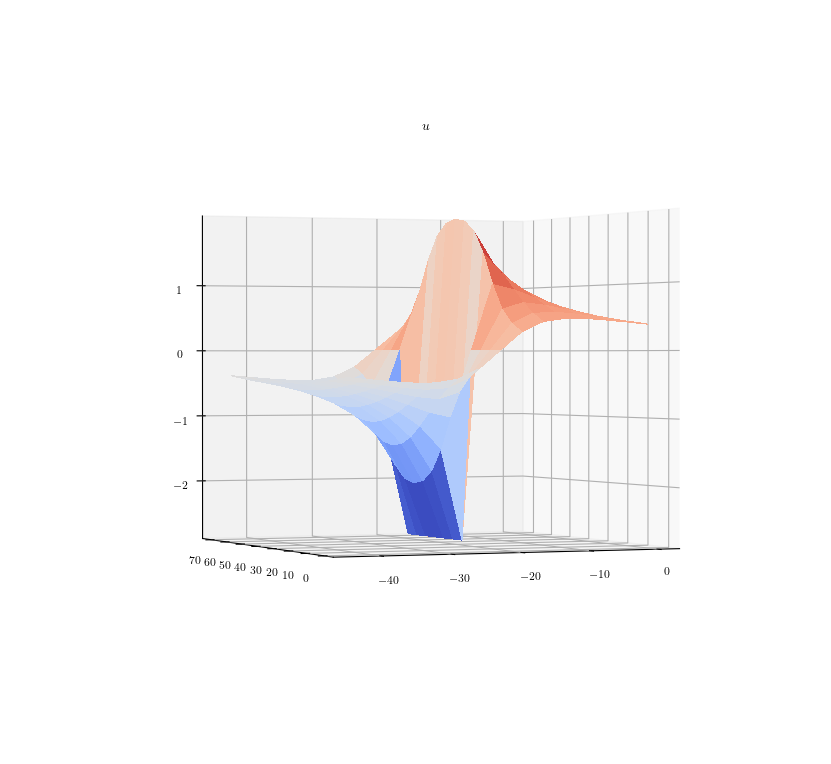
\includegraphics[width=.9\linewidth]{Images/u_dipole_O_arrangement_non_periodic_displacement.png}
\end{center}
Adding in the contribution of the images
\begin{center}
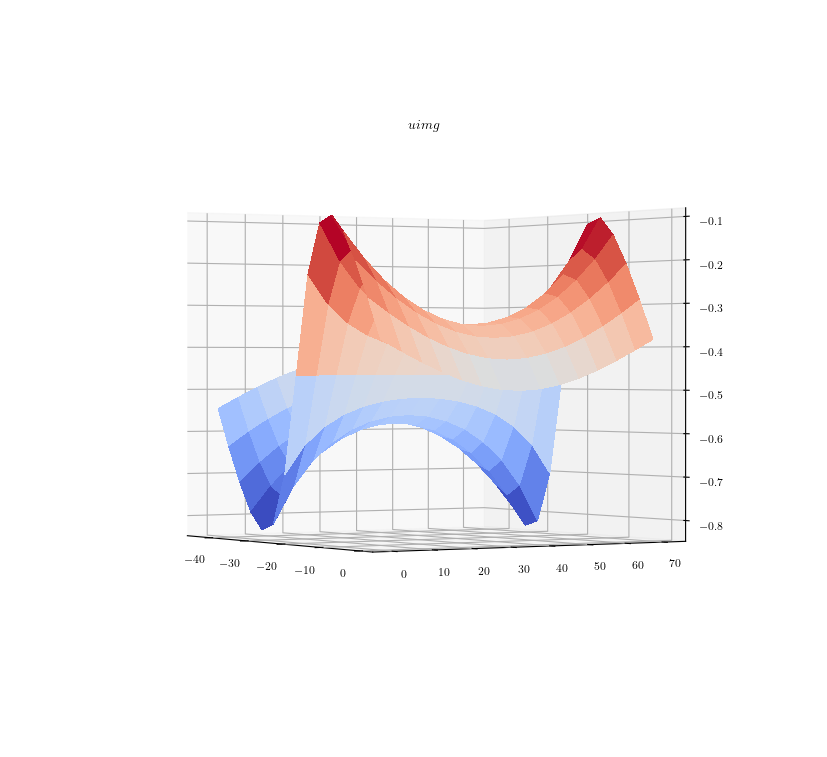
\includegraphics[width=.9\linewidth]{Images/u_image_dipole_O_arrangement.png}
\end{center}
Subtracting from \(u_{\text{sum}}\), the spurious linear displacement:
\begin{center}
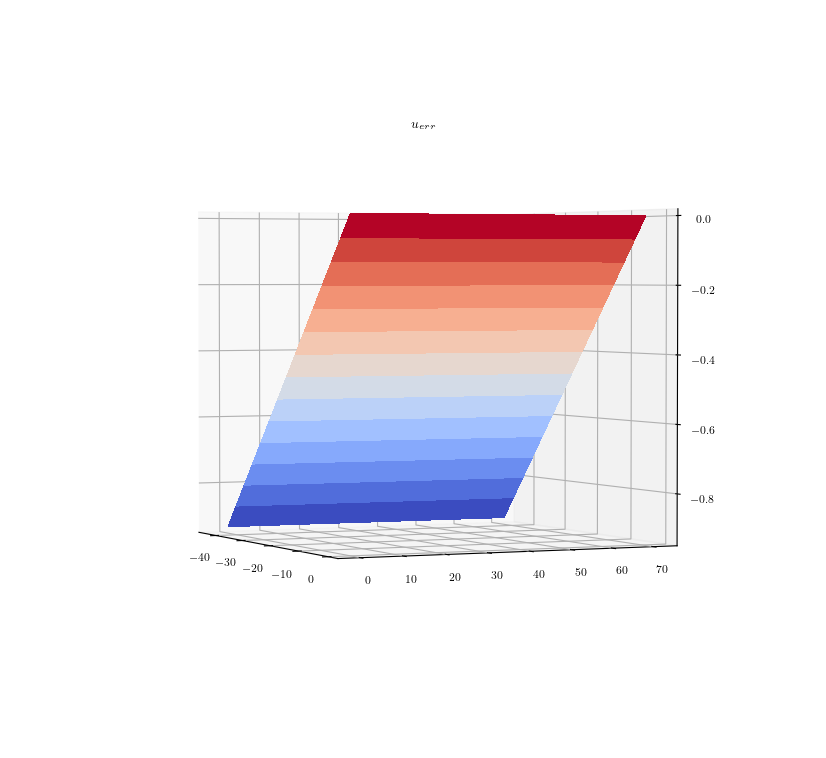
\includegraphics[width=.9\linewidth]{Images/u_err_dipole_O_arrangement.png}
\end{center}
Resulting in the final periodic displacement for the supercell. 
\begin{center}
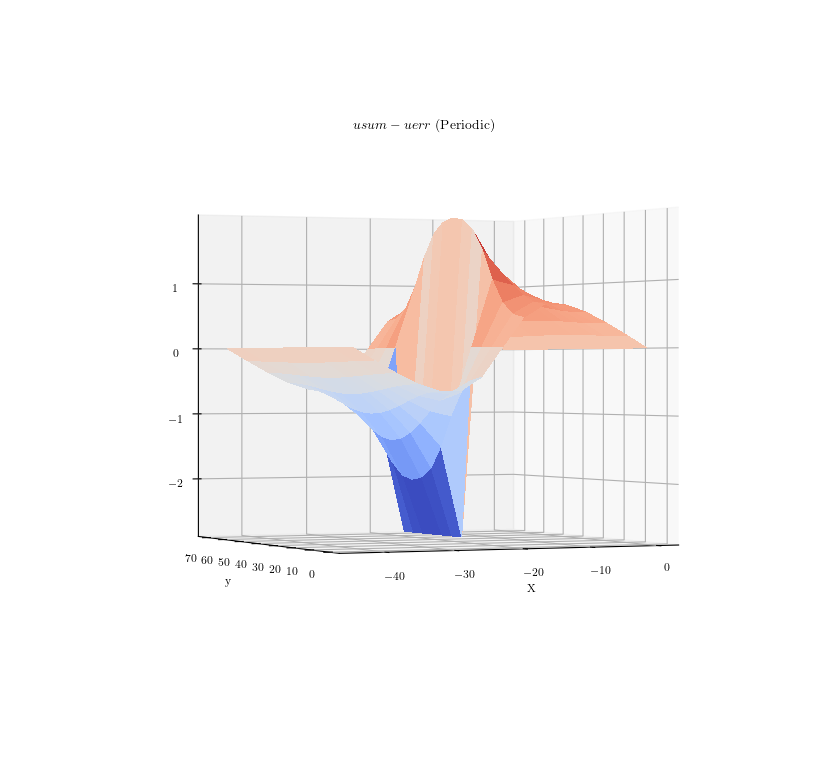
\includegraphics[width=.9\linewidth]{Images/u_dipole_O_arrangement_periodic_displacement.png}
\end{center}
\end{enumerate}

\subsection{Phonons, Elastic Constants and Stability}
\label{sec:orgfc4374c}
\subsubsection{Phonons}
\label{sec:orgc2c87bb}

\begin{enumerate}
\item DFT and TBE Phonons
\label{sec:org1c025c0}
The phonons and q points for the fitting using LDA are here
\begin{center}
\includegraphics[width=.9\linewidth]{/home/tigany/Documents/swarm_fit_ti/phonons_and_strain_derivatives/test_phonopy_conf/dft_results/dft_ctrl_files/from_init/phonon_frequency_calc/hcp_lmf/hcp-band_dos_dft.pdf}
\end{center}
Q point frequencies at M and H are 
\begin{minted}[]{python}
- q-position: [    0.0000000,    0.0000000,    0.5000000 ]
  band:
  - # 1
    frequency:    2.8585871860
  - # 2
    frequency:    2.8585871860
  - # 3
    frequency:    2.8585871860
  - # 4
    frequency:    2.8585871860
  - # 5
    frequency:    5.6670604683
  - # 6
    frequency:    5.6670604683

- q-position: [    0.3300000,    0.3300000,    0.0000000 ]
  band:
  - # 1
    frequency:    4.8064342322
  - # 2
    frequency:    5.5801002486
  - # 3
    frequency:    5.6531673769
  - # 4
    frequency:    6.3665184154
  - # 5
    frequency:    6.4005018626
  - # 6
    frequency:    7.6408237318

\end{minted}
\end{enumerate}

\subsubsection{Elastic constants and Force constant matrix}
\label{sec:org613331d}
\begin{enumerate}
\item Wallace
\label{sec:org42c5371}
\begin{enumerate}
\item Crystal Potential: Introduction
\label{sec:org2c8603f}
\begin{itemize}
\item Since the vibrational energy of a crystal is generally considered to by
small compared to its potential energy, the crystal potential is a first
approximation to the free energy or the internal energy.
\item Ions are labelled by the letters \(M\) and \(N\).
\item Equilibrium positions are given by the vectors \(\mathbf{R}(M)\) and
displacements from equilibrium are denoted by \(\mathbf{U}(M)\).
\item Potential energy of the crystal due to interactions among ions in a
given configuration is given by \(\Phi\), which can be expanded as
\begin{align}
\Phi = \Phi_{0} &+ \sum_{M}\sum_{i} \Phi_{i}(M)U_{i}(M) \\ 
     &+ \frac{1}{2}\sum_{MN}\sum_{ij}\Phi_{ij}(M,N)U_i(M)U_j(N)\\ 
     &+ \frac{1}{3!} \sum_{MNP}\sum_{ijk}\Phi_{ijk}(M,N,P)U_{i}(M)U_{j}(N)U_{k}(P) \\
     &+ \frac{1}{4!} \sum_{MNPQ}\sum_{ijkl}\Phi_{ijkl}(M,N,P,Q)U_{i}(M)U_{j}(N)U_{k}(P)U_{l}(Q) + \dots \\
\end{align}
\item \(\Phi_{i}(M) = \frac{\partial \Phi}{\partial U_{i}(M)}\)
\item \(\Phi_{ij}(M) = \frac{\partial^{2} \Phi}{\partial U_{i}(M)U_{j}(N)}\)
\item These are symmetric in their index pairs; \emph{i.e.} \(\Phi_{ij}(M,N) = \Phi_{ji}(N,M)\)
\item All of the coefficients are functions of the \emph{initial} configuration.
\item This potential is supposed to represent the \emph{entire} energy of the crystal
except for the kinetic energy of the ions.
\item From now on \(M, N\) represent the unit cell and \(\mu, \nu\) represent the
individual ions in a given cell.
\item The total potential of the system plus externally applied forces is
\(\Psi\). For a virtual process where the crystal is deformed while the
externally applies forces are held constant \(\Psi\) is not conserved, if
the forces are changed then it can be conserved. 
\begin{align}
\Psi = \Psi_{0} &+ \sum_{M}\sum_{i}[\Phi_{i}(M) - f_i(M)]U_{i}(M)\\
     &+ \frac{1}{2}\sum_{MN}\sum_{ij}\Phi_{ij}(M,N)U_i(M)U_j(N) \dots
\end{align}
\end{itemize}
\item Stability and the Dynamical Matrix
\label{sec:orged3228b}
\begin{itemize}
\item The equilibrium configuration of ions and external forces is a stable
equilibrium if the total system potential is minimum with respet to
small virtual displacements of the ions from equilirium.
\end{itemize}
\[\Psi = \Psi_{0}+
     \frac{1}{2}\sum_{MN}\sum_{ij}\Phi_{ij}(M,N)U_i(M)U_j(N) + \dots \]
\begin{itemize}
\item The stability condition is if they are positive definite: positive for
any of the values \(U_{i}(M)\), except if they are all 0.
\item The stability condition is:
\[ \sum_{\alpha \beta} \Phi_{\alpha\beta}U_{\alpha}U_{\beta} > 0 \]
\item \(\alpha\), \(\beta \dots\) are indices which refer to the pair  \(Mi\) and
\(>0\) means positive definite (all the eigenvalues are greater than zero).
\item This is only satisfied if the matrix \(\Phi_{\alpha\beta}\) is positive definite
\end{itemize}
\end{enumerate}
\end{enumerate}
\subsubsection{Inner Elastic constants}
\label{sec:org39c42e8}
This is a file which is to evaluate the elastic constants in both relaxed and unrelaxed configurations
According to \cite{Clouet2012} and \cite{Cousins1979}, in a strained hcp lattice there are internal degrees of freedom
that are not accounted for when applying a homogeneous strain.
This is necessary for \(C_{11}\), \(C_{12}\) and \(C_{66}\) elastic constants.
Two of these inner elastic constants, \(e_{11}\), \(e_{11}\), are related to the phonon frequencies of the optical branches at the gamma point.
\[\omega_i = 2  \sqrt{ \Omega  e_{ii} / m }\]
Where \(\Omega = a^2  c  \sqrt{3} / 2\) (The atomic volume), and \(m\) is the mass
The inner elastic constants \(d_{21}\) couples the internal degrees of freedom to the homogeneous strain, leading to a contribution:
\[\delta C_{12} = d_{21}^2 / e_{11}\]
\(C^0_{ij}\) are the unrelaxed elastic constants
The true elastic constants are then given by 
\(C_{11} = C^0_{11} - \delta C_{12}\) 
\(C_{12} = C^0_{11} + \delta C_{12}\) 
\(C_{66} = C^0_{66} - \delta C_{12}\) 
With all others being unchanged 

\begin{enumerate}
\item Sutton
\label{sec:org0151a5a}
Can express the elastic constants as 
\[ C_{ijkl} = \frac{\partial^2 E}{\partial e_{ij}\partial e_{kl}} \]
And also we can express them as 
\[ C_{ikjl} = -\frac{1}{2\Omega} \sum_{p\neq n} \big( X_k^{(p)} - X_k^{(n)} \big) S_{ij}^{(np)}  \big( X_l^{(p)} - X_l^{(n)}  \big)  \]

And to respect the symmetries of the crystal we have 
\begin{align}
 C_{ikjl} = -\frac{1}{8\Omega}  \Big\{ 
    &\sum_{p\neq n}\big( X_k^{(p)} - X_k^{(n)} \big) S_{ij}^{(np)}  \big( X_l^{(p)} - X_l^{(n)}  \big) \\
  + &\sum_{p\neq n}\big( X_i^{(p)} - X_i^{(n)} \big) S_{kj}^{(np)}  \big( X_l^{(p)} - X_l^{(n)}  \big) \\
  + &\sum_{p\neq n}\big( X_k^{(p)} - X_k^{(n)} \big) S_{il}^{(np)}  \big( X_j^{(p)} - X_j^{(n)}  \big) \\
  + &\sum_{p\neq n}\big( X_i^{(p)} - X_i^{(n)} \big) S_{kl}^{(np)}  \big( X_j^{(p)} - X_j^{(n)}  \big)  \Big\},
\end{align}

where \(\Omega\) is the volume of the primitive unit cell and
\[ S_{ij}^{(np)} =  \frac{\partial E}{\partial u_i^{(n)} \partial u_j^{(p)} } \]

If there is more than one atom associated with each lattice site, 
those atoms not on lattice sites may undergo small displacements in addition to those prescribed by the homogeneous strain.
These additional displacements are sometimes called the 'internal strain'. 
Although the strain is stil imposed by displacing atoms at lattice sites, atoms between lattice sites will expreience 
net forces as a result of the strain if they are not at centres of inversion. 
Relaxation of those forces reduces the energy of the homogeneously strained crystal, and therefore it affects the calculated elastic constants.
\end{enumerate}
\subsubsection{Notes on Thermodynamics and Stability}
\label{sec:org0f28478}

\begin{enumerate}
\item Wallace 1972
\label{sec:org4622896}
\begin{itemize}
\item For hexagonal materials, there are general stability requirements:
\begin{itemize}
\item \(C_{11} - C_{12} > 0\)
\item \(C_{11} + C_{12} + C_{33} > 0\)
\item \(( C_{11} + C_{12} ) C_{33} - 2C_{13}^{2} > 0\)
\item \(C_{44} > 0\)
\item \(C_{66} = \frac{1}{2}(C_{11} - C_{12}) > 0\)
\item \(( C_{11} + C_{12} )C_{33} > 0\)
\item \(C_{11} + C_{12} > 0\)
\item \(C_{33} > 0\)
\item \(C_{11} > 0\)
\end{itemize}
\item The equilibrium configuration of ions plus external forces is a stable
equilibrium if the total system potential \(\Psi\) is minimum with respect
to small virtual displacements of dions from equilibrium.
\item Cauchy relations (at least in the cubic case) will be destroyed if
non-central forces are included in the crystal potential.
\end{itemize}

\item Fast, Will, Johansson: Elastic constants in hexagonal transition metals
\label{sec:org0fb2d80}

\begin{enumerate}
\item Cauchy Relations
\label{sec:org6cfe983}
\begin{itemize}
\item Cauchy relations for hexagonal materials:
\begin{itemize}
\item \(C_{13} = C_{44}\)
\item \(C_{12} = C_{66} = \frac{1}{2}(C_{11} - C_{12})\)
\end{itemize}
\item These only are meant to hold for central forces.
\item These Cauchy forces have been shown to hold more in hexagonal materials
rather than cubic ones.
\item In cubic materials sometimes one finds \(C_{44}\) four times smaller than
\(C_{12}\).
\item They showed the Cauchy ratios:
\begin{itemize}
\item \(C_{12}/C_{66}\)
\item \(C_{13}/C_{44}\)
\end{itemize}
\item The Cauchy relations were close to 1 apart from calculations with Co, Zr and
Ti, where it was closer to 2.
\item These are smaller than the \(3/4\) times deviations in cubic crystals.
\end{itemize}

\item Normalised elastic constant
\label{sec:orge43ba64}
\begin{itemize}
\item To investigate Cauchy relations fully they used a normalised elastic constant which
was obtained by dividiing by the bulk modulus: \(C'_{ij} = C_{ij}/B\)
\item It becomes easier to study trends as one is normlising the
interatomic forces with an average restoring force of the system,
when dividing by the bulk modulus.
\item Suggest that the hexagonal materials are quite isotropic.
\end{itemize}
\end{enumerate}

\item Calculation of elastic constants by various means
\label{sec:org2b0cc79}
\begin{enumerate}
\item Calculation by derivative of energy with strain
\label{sec:orgf075c8f}
One way to calculate the elastic constants is to take derivatives of the elastic energy density with respect to strain
\[ C_{ijkl} = \frac{1}{2}\frac{\partial E}{ \partial e_{ij} \partial
e_{kl} } \]
\begin{enumerate}
\item Results
\label{sec:org760fe74}
\begin{enumerate}
\item Correct Strain Derivative
\label{sec:org56fd21e}
Initially it was thought that checking if the 9x9 matrix of elastic constants was positive definite was enough
to ascertain the stability of the crystal, but it seems that acutally all of the stability criteria
are satisfied and that actually it is the 6x6 elastic constant matrix that needs to be positive definite,

However Phonopy does still get soft modes at gamma and so it is perplexing why this might be happening. 
Phonopy might be interfering with the crystal symmetry.
There are two eigenvalues from the 9x9 matrix that are usually the same and negative, so this might be a reason
as to why there is a soft mode, but this is uncertain. One may have to construct the dynamical matrix by hand. 

I'd argue that taking the derivatives is quite accurate. We reproduce c44, the only one of tony's set of strains
that is symmetric about zero strain, within a few percent (34.9 from derivative to 38.1 GPa from the fifth order polynomial).
Using a second order routine of \(h=0.001\) we obtain:
\begin{minted}[]{python}

# Full matrix :

  156.2634    62.2392    55.7344    -0.0000     0.0000     0.0000     0.0000    -0.0000     0.0000
   62.2392   156.4112    55.5866    -0.0000     0.0000     0.0000     0.0000    -0.0000     0.0000
   55.7344    55.5866   157.1504     0.0000     0.0000     0.0000     0.0000     0.0000     0.0000
   -0.0000    -0.0000     0.0000    34.8894     0.0000     0.0000    34.8894     0.0000     0.0000
    0.0000     0.0000     0.0000     0.0000    32.8198     0.0000     0.0000    34.8894     0.0000
    0.0000     0.0000     0.0000     0.0000     0.0000    47.0120     0.0000     0.0000    47.0120
    0.0000     0.0000     0.0000    34.8894     0.0000     0.0000    32.8198     0.0000     0.0000
   -0.0000    -0.0000     0.0000     0.0000    34.8894     0.0000     0.0000    34.8894     0.0000
    0.0000     0.0000     0.0000     0.0000     0.0000    47.0120     0.0000     0.0000    47.0120

With eigenvalues:

272.3589+0.0000j 103.3698+0.0000j 94.0963+0.0000j 94.0240+0.0000j 68.7593+0.0000j 68.7593+0.0000j -1.0501+0.0000j -1.0501-0.0000j 0.0000+0.0000j

So the matrix is not positive definite although it satisfies the stability criteria

C_11 156.2634
C_33 157.1504
C_44 34.8894
C_12 62.2392
C_13 55.7344

C_11 - C_12 > 0 
 True
 C_11 + C_12 + C_33 > 0 
 True
( C_11 + C_12 ) * C_33 - 2 * C_13**2 > 0 
 True
C_44 > 0 
 True
(C_11 - C_12) > 0
 True
( C_11 + C_12 )*C_33 > 0 
 True
C_11 + C_12 > 0
  True
C_33 > 0
 True
C_11 > 0
 True

\end{minted}

The aforementioned actually has bzjob=1\ldots{}
Letting bzjob=0 we have very slightly different results 
\begin{minted}[]{python}
C_11 156.55906025190512
C_33 157.15040703252774
C_44 34.88946007560986
C_12 62.091411998201686
C_13 55.58659740765988
\end{minted}


Using a fourth order mixed derivative we have a similar story:

\begin{minted}[]{python}

  156.2100    62.2926    55.8206    -0.0000     0.0000     0.0000     0.0000    -0.0000    -0.0329
   62.2926   156.3496    55.5784    -0.0000     0.0000    -0.0575     0.0000    -0.0000    -0.0575
   55.8206    55.5784   157.1464     0.0000     0.0000     0.0287     0.0000     0.0000     0.0287
   -0.0000    -0.0000     0.0000    34.7662     0.0000     0.0000    34.8976     0.0000     0.0000
    0.0000     0.0000     0.0000     0.0000    32.7048     0.0000     0.0000    34.8976     0.0000
    0.0000    -0.0575     0.0287     0.0000     0.0000    46.8970     0.0000     0.0000    46.8970
    0.0000     0.0000     0.0000    34.8976     0.0000     0.0000    32.7048     0.0000     0.0000
   -0.0000    -0.0000     0.0000     0.0000    34.8976     0.0000     0.0000    34.7580     0.0000
   -0.0329    -0.0575     0.0287     0.0000     0.0000    46.8970     0.0000     0.0000    46.8970

With eigenvalues
  272.4062   103.3167    93.9916    93.7855    -0.0000    -1.1813    -1.1773    68.6483    68.6441

so the matrix is not positive definite

C_11 - C_12 > 0 
 True
 C_11 + C_12 + C_33 > 0 
 True
( C_11 + C_12 ) * C_33 - 2 * C_13**2 > 0 
 True
C_44 > 0 
 True
(C_11 - C_12) > 0
 True
( C_11 + C_12 )*C_33 > 0 
 True
C_11 + C_12 > 0
  True
C_33 > 0
 True
C_11 > 0
 True

\end{minted}

With bzjob=0 we have
\begin{minted}[]{python}
C_11 156.68225749754902
C_33 157.08880840888514
C_44 34.88946007629375
C_12 62.12426459729613
C_13 55.64408945578736
\end{minted}
with none of the spurious off diagonal terms. 
\item Miscellaneous
\label{sec:org21830d6}
These are the results for the model from December by tony. 
\begin{minted}[]{bash}

Elastic constant matrix Ryd/AA**3:
 [[2.2272  0.27192 0.80071 0.16768 0.      0.72153 0.0575  0.17501 0.     ]
 [0.27192 0.49531 0.10444 0.      0.10815 0.      0.02675 0.      0.     ]
 [0.80071 0.10444 1.15753 0.00964 0.      0.      0.21149 0.31484 0.00912]
 [0.16768 0.      0.03253 0.67398 0.      0.      0.      0.04262 0.0558 ]
 [0.      0.10815 0.      0.      0.3322  0.08569 0.      0.61174 0.     ]
 [0.64789 0.      0.      0.      0.06787 0.51815 0.00377 0.      0.11769]
 [0.0575  0.04526 0.19313 0.05313 0.      0.00377 0.7419  0.      0.     ]
 [0.13481 0.      0.35608 0.04262 0.77688 0.      0.      2.24564 0.     ]
 [0.      0.      0.00912 0.0558  0.      0.      0.0053  0.01619 0.0823 ]]


\end{minted}

This seems to be a quite noisy method\ldots{} 
Using the amplitude of the strains as \(h=0.001\) to calculate the mixed
derivatives we have:
\begin{minted}[]{python}
array([[122.3759,   5.5439,  43.119 ,   6.1599,  16.0156,  65.2945,   6.1599,  14.5783,   3.0799],
       [  5.5439,  12.1144,   0.    ,   0.    ,   5.9545,   0.    ,  10.6771,  13.141 ,   5.9545],
       [ 43.119 ,   0.    , 131.8211,  35.3165,   0.    ,  28.3354,   0.    ,   0.    ,   0.    ],
       [  6.1599,   0.    ,  32.4419,  21.9702,   0.    ,   8.8291,   0.    ,   0.    ,   0.    ],
       [  0.    ,   5.9545,   0.    ,   0.    ,   4.5172,   2.8746,   2.8746,  39.8338,   1.6426],
       [ 57.492 ,   0.    ,  28.3354,   8.8291,   1.232 ,   0.    ,  14.989 ,  29.362 ,   0.    ],
       [  6.1599,   0.    ,   5.7492,   0.    ,   2.8746,  14.989 ,  20.3275,   0.    ,   0.    ],
       [ 14.5783,  13.141 ,   0.    ,   0.    ,  35.1112,  29.362 ,   0.    , 326.8834,   1.232 ],
       [  4.7226,   4.3119,   0.    ,   0.    ,   1.6426,   0.    ,   0.    ,   0.4107,   0.    ]])

>>> np.linalg.eigvals( ect )
array([336.8415, 194.2468,  93.2178, -30.711 ,  20.7759,  16.3516,  12.3729,  -1.8979,  -1.188 ])

\end{minted}
Using fourth order mixed derivatives for the strain:
\begin{minted}[]{python}
array([[ 133.05,  14.784,  56.055,  17.453,  2.6693e+00,  3.2647e+01, -1.2320e+00, -1.0266e+01, -4.1066e-01],
       [ 14.784,  32.853,  8.8292, -28.746,  2.2176e+01, -9.1184e-09, -1.2320e+00, -1.1498e+01, -1.7658e+01],
       [ 56.055,  8.8292,  76.588, -1.4373,  1.6632e+01, -2.0944e+01,  1.7864e+01,  1.0472e+01,  2.8495e-10],
       [ 17.453, -2.8746, -1.4373,  43.940, -1.0472e+01, -1.7658e+01, -1.1909e+01, -3.2853e+00, -4.5172e+00],
       [ 2.6693,  22.176,  16.632, -10.472,  25.255,  1.0266e+01, -2.6282e+01,  5.5849e+01, -1.0061e+01],
       [ 32.647,   1e-9,   -20.944, -17.658,  1.0266e+01,  43.119,  1.8522e-08,  4.5172e+00,  7.3918e+00],
       [-1.2320, -1.2320,  17.864, -11.909, -2.6282e+01,  1.8522e-08,  57.492, -5.4412e+01, -2.8495e-10],
       [-10.266, -11.498,  10.472, -3.2853,  5.5849e+01,  4.5172e+00, -5.4412e+01,  133.05, -2.0533e-01],
       [-0.4106, -17.658,  1e-10, -4.5172, -1.0061e+01,  7.3918e+00, -2.8495e-10, -2.0533e-01,  27.103e+01]])

array([[ 133.05,  14.784,  56.055,  17.453,  0,    0,    0,    0,    0],
       [ 14.784,  32.853,  8.8292, -28.746,  0,    0,    0,    0,    0],
       [ 56.055,  8.8292,  76.588, -1.4373,  0,    0,    0,    0,    0],
       [ 17.453, -2.8746, -1.4373,  43.940,  0,    0,    0,    0,    0],
       [ 2.6693,  22.176,  16.632, -10.472,  25.255,  0,    0,    0,    0],
       [ 32.647,   1e-9,   -20.944, -17.658,  1.0266e+01,  43.119,   0,    0,    0],
       [-1.2320, -1.2320,  17.864, -11.909, -2.6282e+01,  1.8522e-08,  57.492,  0,    0],
       [-10.266, -11.498,  10.472, -3.2853,  5.5849e+01,  4.5172e+00, -5.4412e+01,  133.05,  0],
       [   0,      0,      0,      0,      0,      0,      0,      0,     27.103e+01]])

\end{minted}
\end{enumerate}
\end{enumerate}
\item Calculation using fifth order polynomials
\label{sec:org153230f}
\begin{enumerate}
\item Results: December 2018
\label{sec:orge50467e}
\begin{enumerate}
\item Applied Strains in code
\label{sec:orgdac538c}
\begin{center}
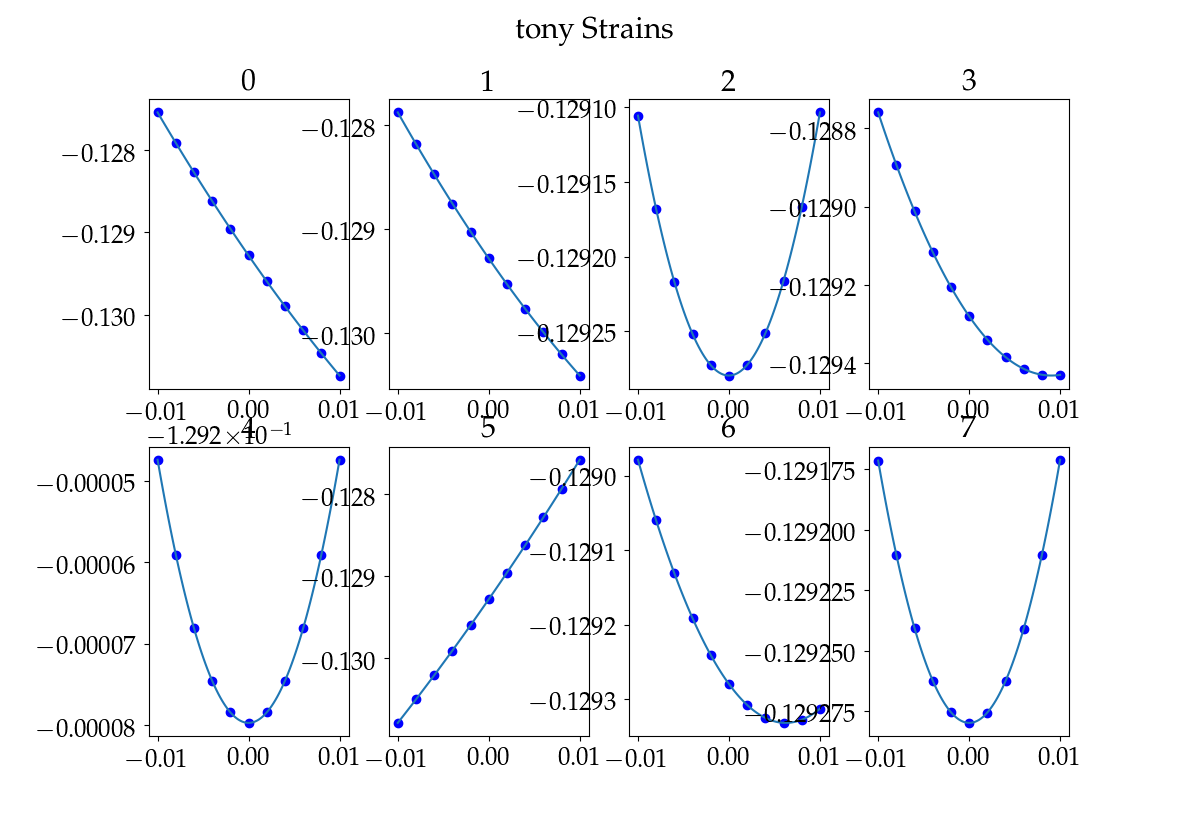
\includegraphics[width=.9\linewidth]{Images/tony_real_strains_2018_12_22.png}
\end{center}
\begin{minted}[]{python}
Elastic Constants: Tony Strains


C11 =  165.8231485457,   C11_exp =  176.1000000000 
C33 =  164.5632628633,   C33_exp =  190.5000000000 
C44 =  38.1494487390,    C44_exp =  50.8000000000  
C66 =  207.5028445231,   C66_exp =  44.6000000000  
C12 = -249.1825405004,   C12_exp =  86.9000000000  
C13 = -273.1296728747,   C13_exp =  68.3000000000  
K   = -1094.6742125447,  K_FR    =  109.9666666667 
R   =  669.1429126353,   R_FR    =  61.8000000000  
H   =  634.1671283357,   H_FR    =  45.9650000000  
\end{minted}

\begin{center}
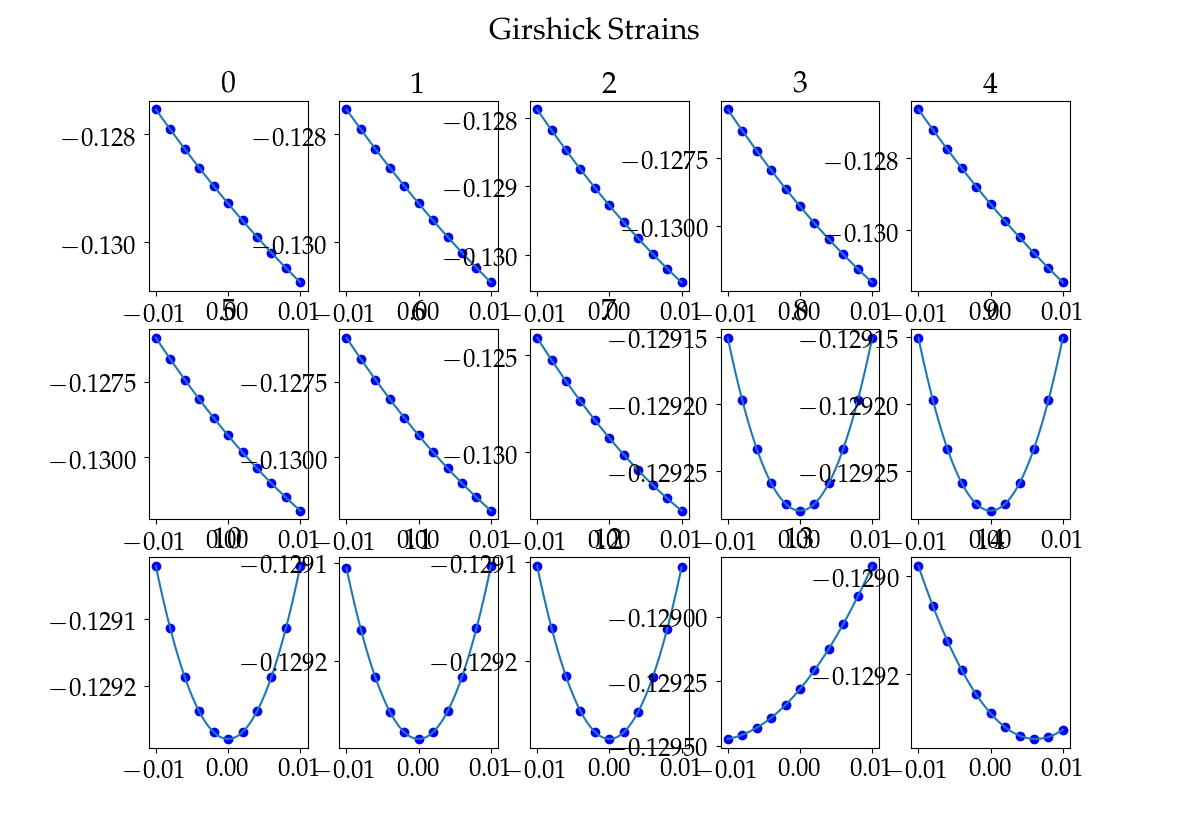
\includegraphics[width=.9\linewidth]{Images/girshick_real_strains_2018_12_22.png}
\end{center}

\begin{minted}[]{python}
Elastic Constants: Girshick Routine Applied Strains 


C11 =  165.8623476695,   C11_exp =  176.1000000000 
C33 =  164.5632628633,   C33_exp =  190.5000000000 
C44 =  38.1796557562,    C44_exp =  50.8000000000  
C66 =  51.8860924371,    C66_exp =  44.6000000000  
C12 = -10383.7435816516, C12_exp =  86.9000000000  
C13 = -9548.9999553500,  C13_exp =  68.3000000000  
K   =  93.6545272856,    K_FR    =  109.9666666667 
R   =  55.7940512318,    R_FR    =  61.8000000000  
H   =  52.8336415119,    H_FR    =  45.9650000000  
\end{minted}

\item Applied Strains in tbe
\label{sec:org00e9d28}

Girshick 

\begin{center}
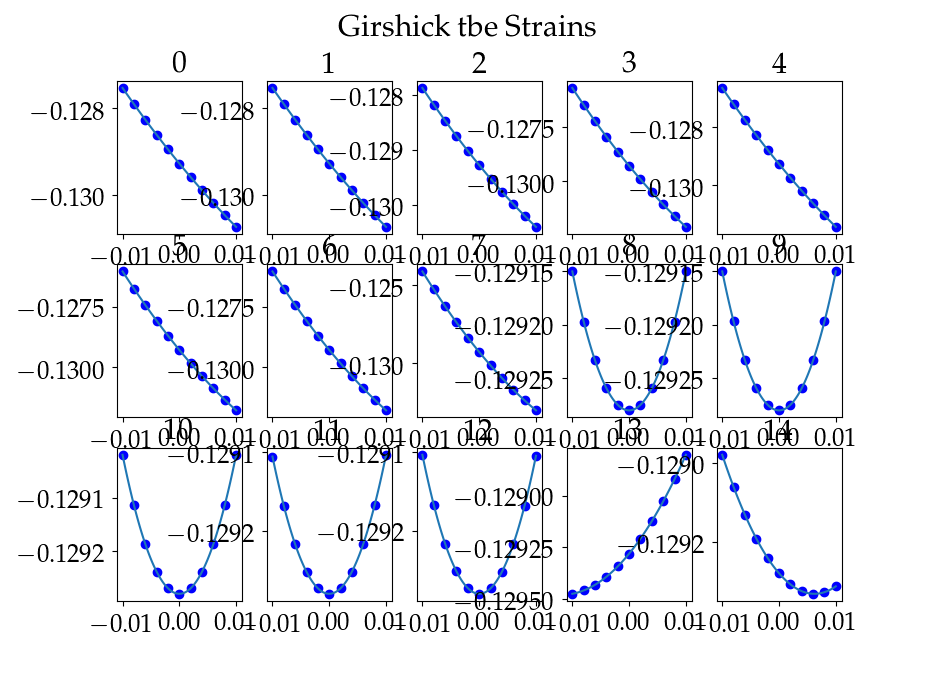
\includegraphics[width=.9\linewidth]{Images/girshick_tbe_strains_2018_12_22.png}
\end{center}
\begin{minted}[]{python}
C11 =  165.8623476695,   C11_exp =  176.1000000000
C33 =  164.5632628633,   C33_exp =  190.5000000000
C44 =  38.1796557562,   C44_exp =  50.8000000000
C66 =  51.8860924371,   C66_exp =  44.6000000000
C12 = -10383.7436103689,   C12_exp =  86.9000000000
C13 = -9548.9962292795,   C13_exp =  68.3000000000
K =  93.6561928893,   K_exp =  109.9666666667
R =  55.7940512318,   R_exp =  61.8000000000
H =  52.8336415119,   H_exp =  45.9650000000

\end{minted}

\begin{center}
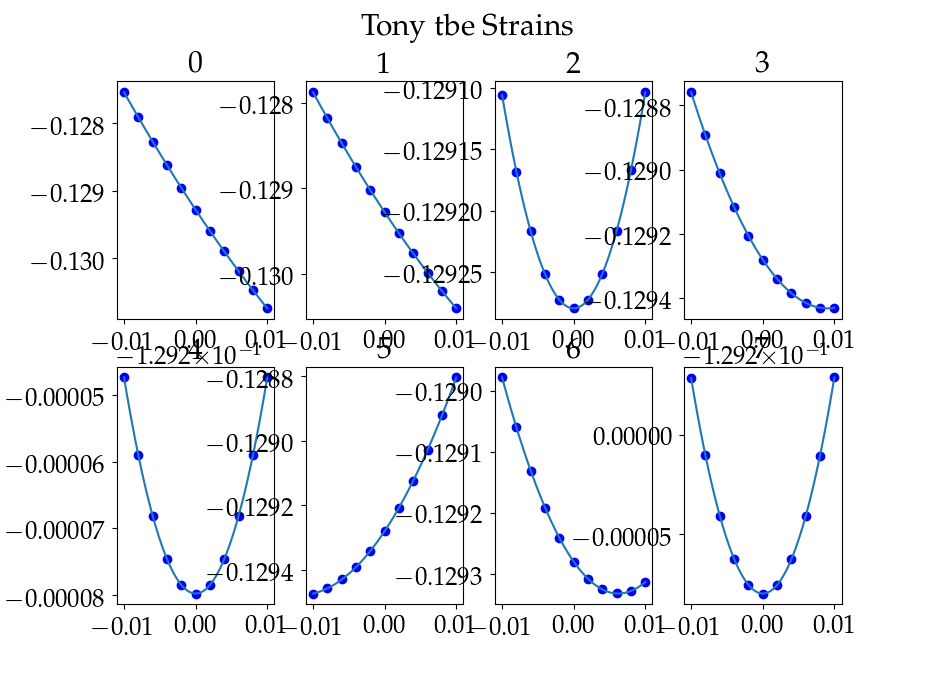
\includegraphics[width=.9\linewidth]{Images/tony_tbe_strains_2018_12_22.png}
\end{center}
\begin{minted}[]{python}
C11 =  165.8231485457,   C11_exp =  176.1000000000
C33 =  164.5632628633,   C33_exp =  190.5000000000
C44 =  38.1494487390,   C44_exp =  50.8000000000
C66 =  207.5028445231,   C66_exp =  44.6000000000
C12 = -249.1825405004,   C12_exp =  86.9000000000
C13 = -273.1296728747,   C13_exp =  68.3000000000
K = -1094.6742125447,   K_exp =  109.9666666667
R =  669.1429126353,   R_exp =  61.8000000000
H =  634.1671283357,   H_exp =  45.9650000000 

\end{minted}
\end{enumerate}


\item Unordered Results
\label{sec:org7441a2c}
\begin{center}
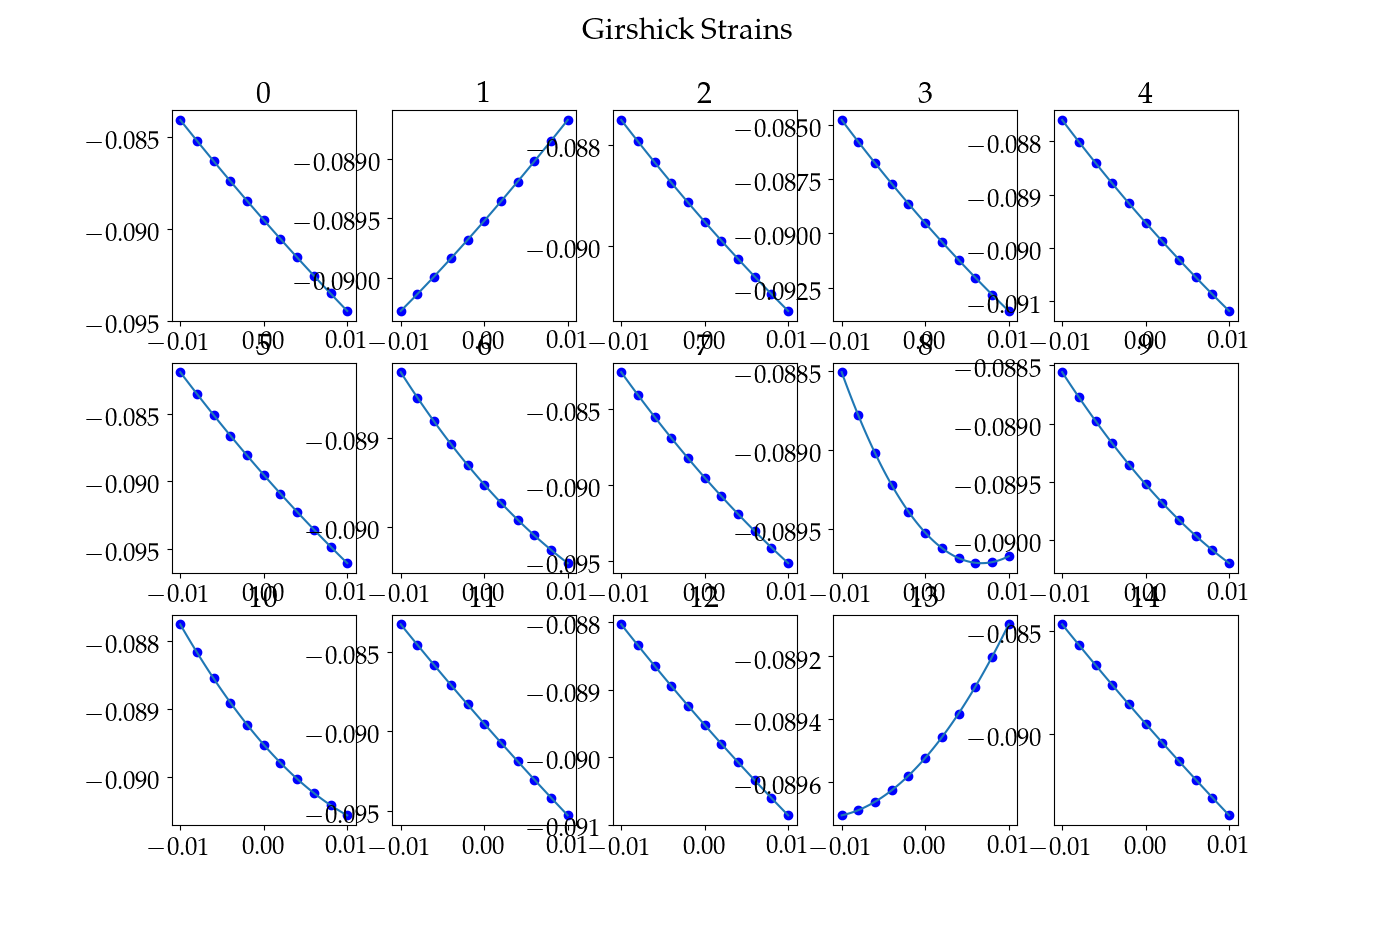
\includegraphics[width=.9\linewidth]{Images/girshickstrains.png}
\end{center}
\begin{minted}[]{python}
C11 =  173.9155276479,   C11_exp =  176.1000000000
C33 =  147.9542064528,   C33_exp =  190.5000000000
C44 =  69.6511083920,   C44_exp =  50.8000000000
C66 =  46.6885793926,   C66_exp =  44.6000000000
C12 = -10950.9356585199,   C12_exp =  86.9000000000
C13 = -9302.3428901998,   C13_exp =  68.3000000000
K =  86.0339496031,   K_FR =  109.9666666667
R =  47.9671492728,   R_FR =  61.8000000000
H =  74.5803389724,   H_FR =  45.9650000000
\end{minted}




\begin{center}
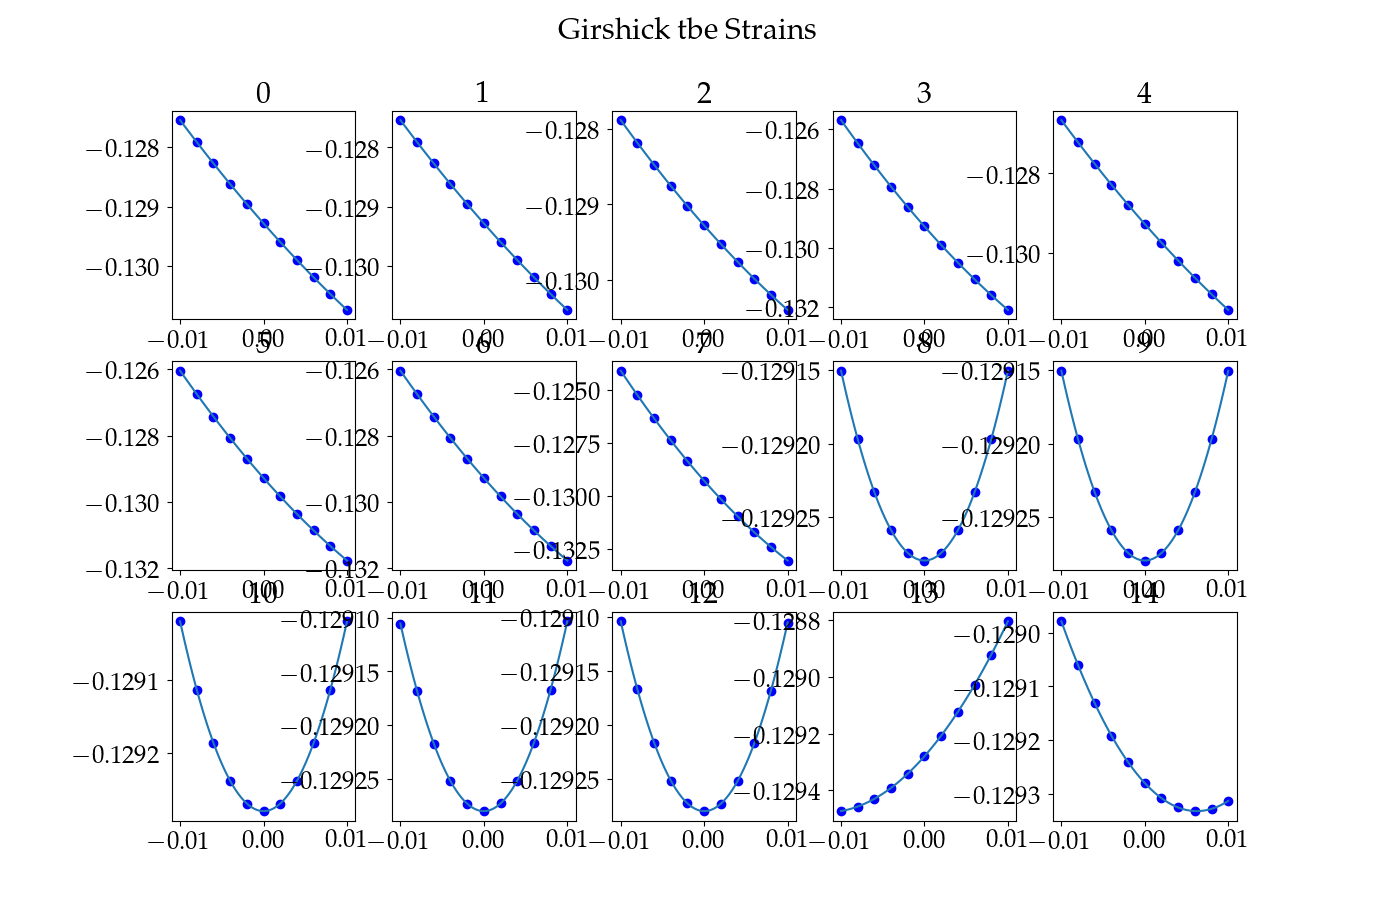
\includegraphics[width=.9\linewidth]{Images/girshicktbestrains.png}
\end{center}

\begin{minted}[]{python}
C11 =  165.8623476701,   C11_exp =  176.1000000000
C33 =  164.5632628639,   C33_exp =  190.5000000000
C44 =  38.1796557563,   C44_exp =  50.8000000000
C66 =  51.8860924373,   C66_exp =  44.6000000000
C12 = -10383.7436104020,   C12_exp =  86.9000000000
C13 = -9548.9962293122,   C13_exp =  68.3000000000
K =  93.6561928893,   K_FR =  109.9666666667
R =  55.7940512319,   R_FR =  61.8000000000
H =  52.8336415120,   H_FR =  45.9650000000

\end{minted}

\begin{center}
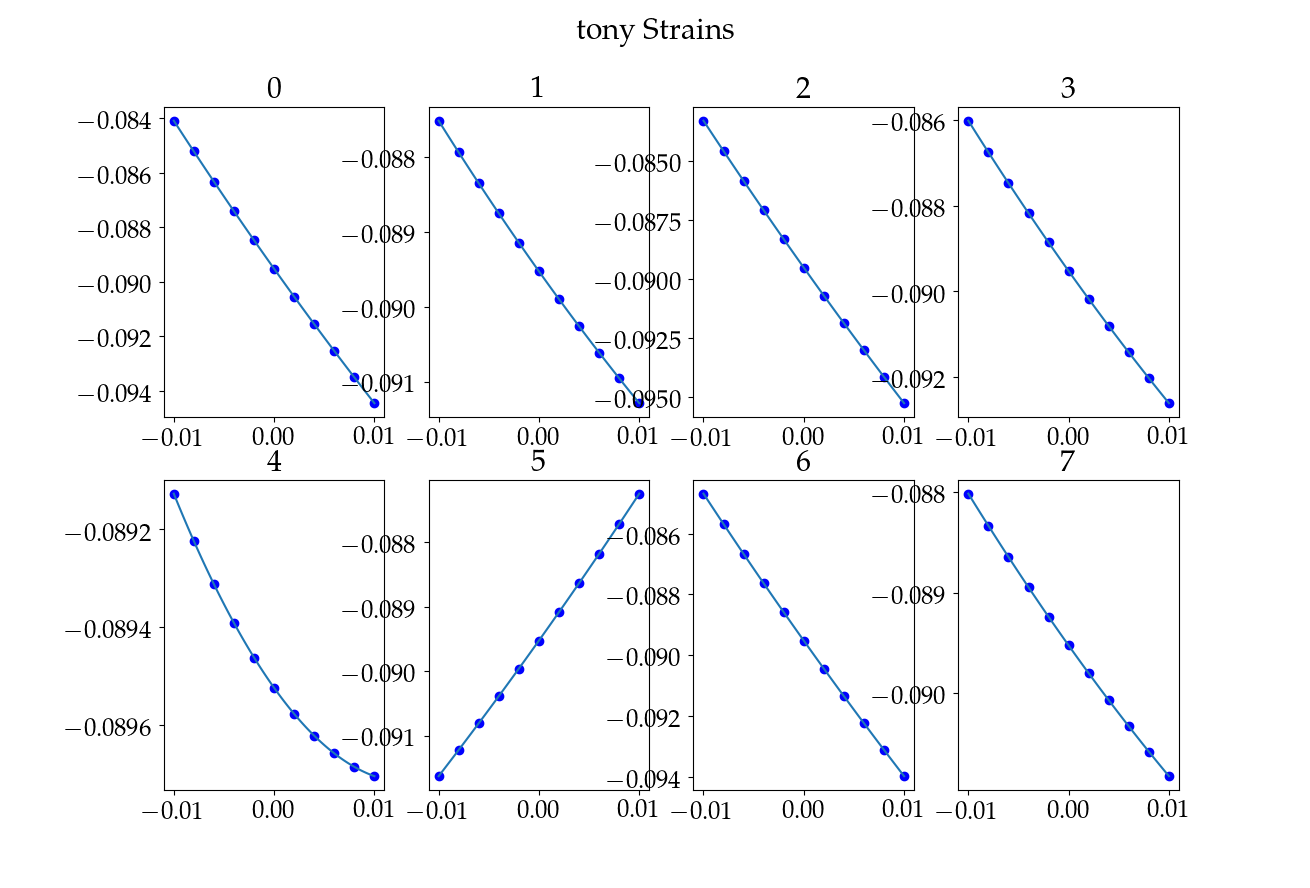
\includegraphics[width=.9\linewidth]{Images/tonystrains.png}
\end{center}
\begin{minted}[]{python}
C11 =  294.0060923538,   C11_exp =  176.1000000000
C33 =  147.9542064528,   C33_exp =  190.5000000000
C44 =  127.6805919606,   C44_exp =  50.8000000000
C66 =  284.0959508096,   C66_exp =  44.6000000000
C12 = -274.1858092654,   C12_exp =  86.9000000000
C13 = -283.8196185256,   C13_exp =  68.3000000000
K = -947.6837014728,   K_FR =  109.9666666667
R =  725.5035850482,   R_FR =  61.8000000000
H =  820.5917855837,   H_FR =  45.9650000000

\end{minted}

\begin{center}
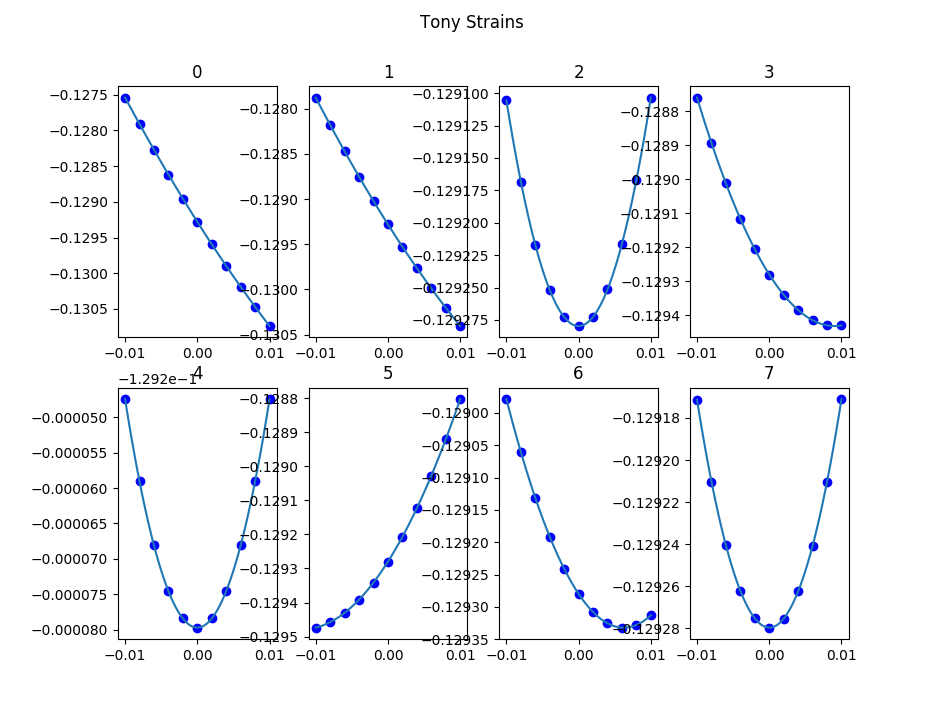
\includegraphics[width=.9\linewidth]{Images/applied_tony_strains.png}
\end{center}
\begin{minted}[]{python}


C11 =  3439.0436276515,   C11_exp =  176.1000000000
C33 =  3704.2209613709,   C33_exp =  190.5000000000
C44 =  4786.2106820819,   C44_exp =  50.8000000000
C66 =  4676.2088087745,   C66_exp =  44.6000000000
C12 = -5913.3739898976,   C12_exp =  86.9000000000
C13 = -5235.9381795662,   C13_exp =  68.3000000000
K = -22188.1924813862,   K_FR =  109.9666666667
R =  12938.9321393802,   R_FR =  61.8000000000
H =  13756.2028545877,   H_FR =  45.9650000000

\end{minted}
\begin{center}
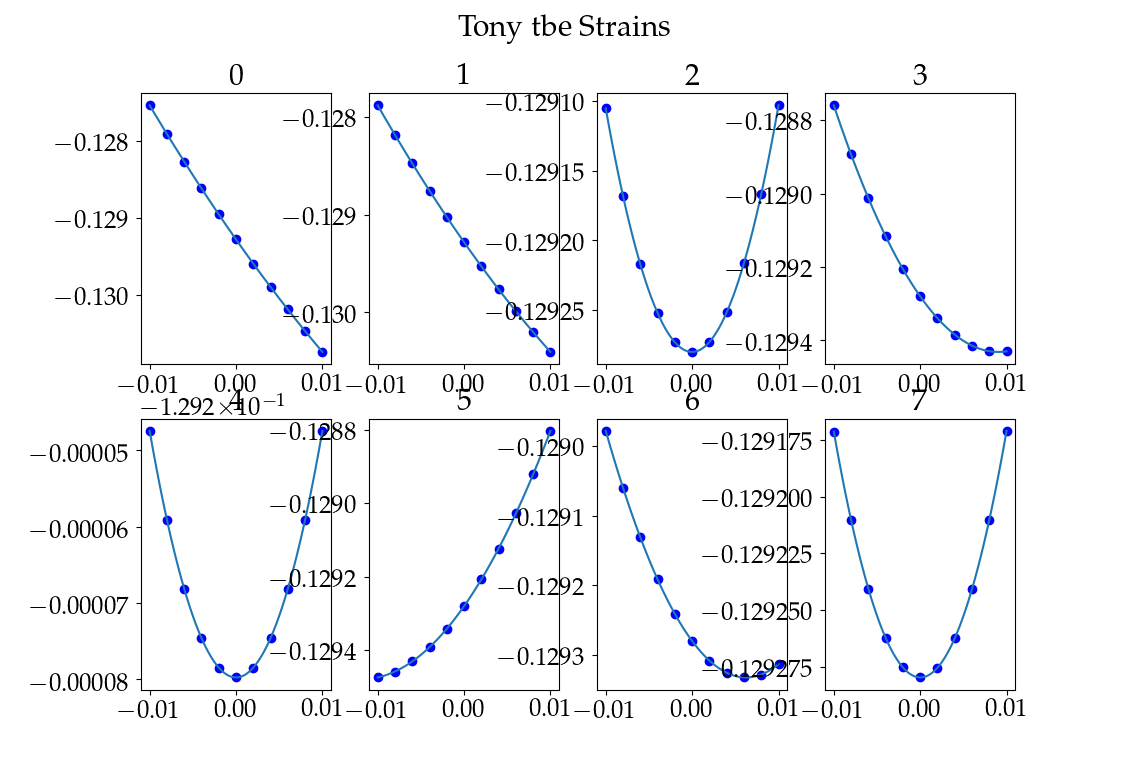
\includegraphics[width=.9\linewidth]{Images/tonytbestrains.png}
\end{center}
\begin{minted}[]{python}
C11 =  165.8231485464,   C11_exp =  176.1000000000
C33 =  164.5632628639,   C33_exp =  190.5000000000
C44 =  38.1494487394,   C44_exp =  50.8000000000
C66 =  207.5028445236,   C66_exp =  44.6000000000
C12 = -249.1825405007,   C12_exp =  86.9000000000
C13 = -273.1296728744,   C13_exp =  68.3000000000
K = -1094.6742125423,   K_FR =  109.9666666667
R =  669.1429126355,   R_FR =  61.8000000000
H =  634.1671283369,   H_FR =  45.9650000000 

\end{minted}


\item Girshick Routines
\label{sec:org53774e9}
This was done by using the methods implemented by Girshick 
\begin{minted}[]{python}
C11 =  174.6582002879,   C11_exp =  176.1000000000
C33 =  148.5838047109,   C33_exp =  190.5000000000
C44 =  69.8223407219,   C44_exp =  50.8000000000
C66 =  46.7301800073,   C66_exp =  5586.2392851153
C12 = -10997.8203699426,   C12_exp =  86.9000000000
C13 = -9342.8091038253,   C13_exp =  68.3000000000
K =  85.9105417657,   K_FR =  109.9666666667
R =  48.5317889633,   R_FR =  61.8000000000
H =  74.1393560210,   H_FR =  45.9650000000 

\end{minted}
Implementing them using the tbe methods we have 
\begin{minted}[]{python}
C11 =  165.8623476701,   C11_exp =  176.1000000000
C33 =  164.5632628639,   C33_exp =  190.5000000000
C44 =  38.1796557563,   C44_exp =  50.8000000000
C66 =  51.8860924373,   C66_exp =  44.6000000000
C12 = -10383.7436104020,   C12_exp =  86.9000000000
C13 = -9548.9962293122,   C13_exp =  68.3000000000
K =  93.6561928893,   K_FR =  109.9666666667
R =  55.7940512319,   R_FR =  61.8000000000
H =  52.8336415120,   H_FR =  45.9650000000
\end{minted}
\begin{center}
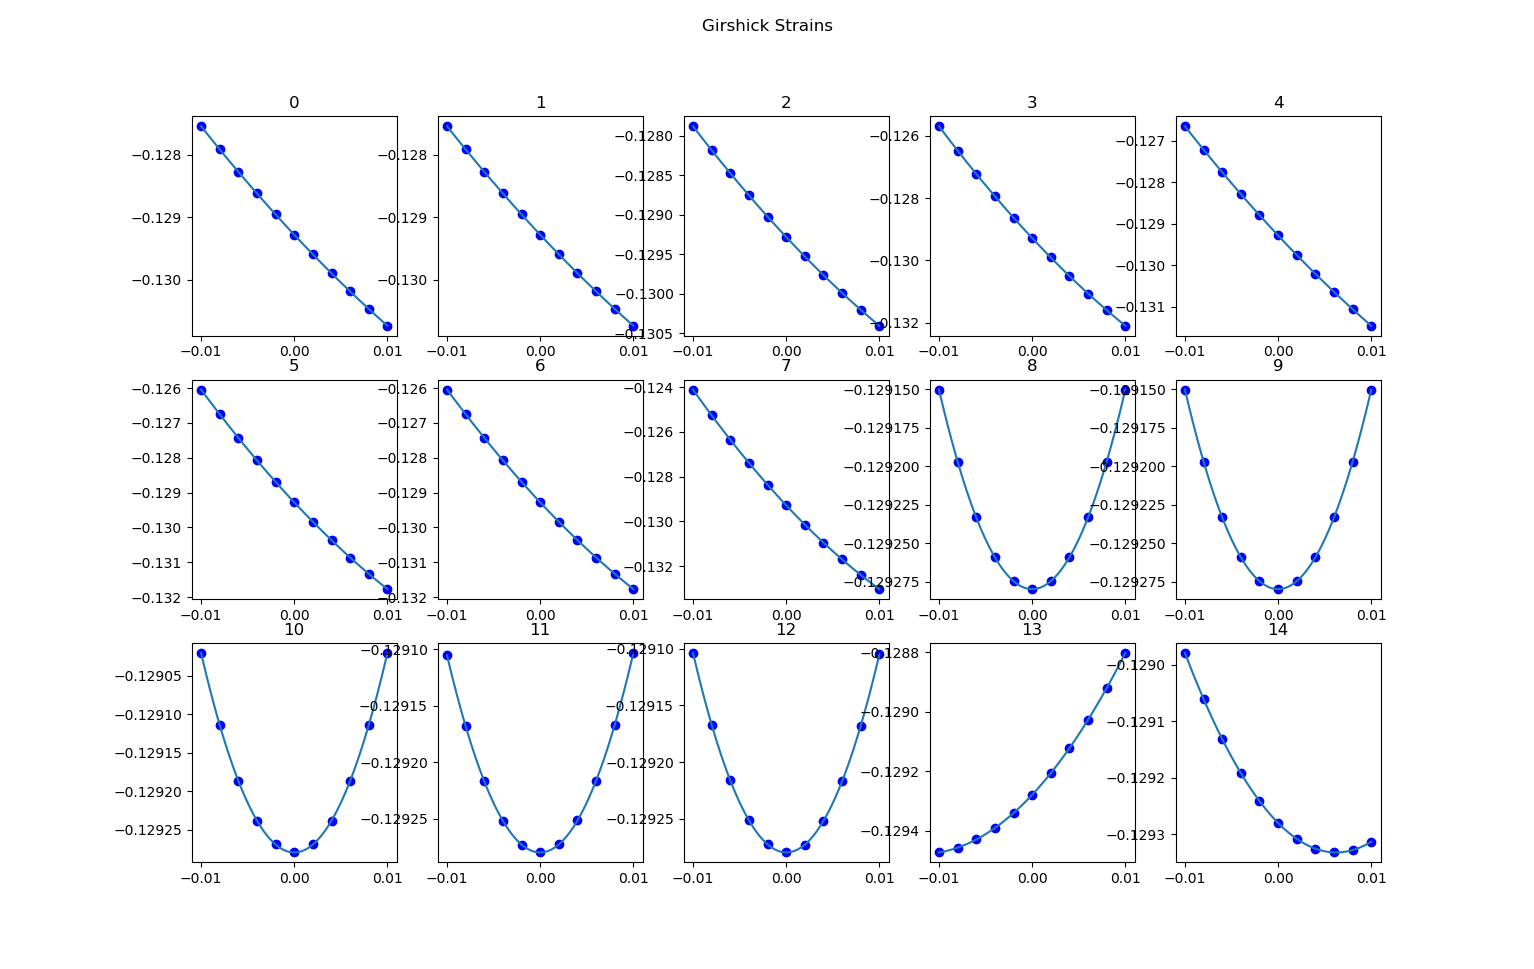
\includegraphics[width=.9\linewidth]{Images/tbe_routine_girshick_strains.png}
\end{center}

\item Tony Routines
\label{sec:org2a1f90d}
With tony's routines we have 
\begin{minted}[]{python}
C11 =  165.8231485464,   C11_exp =  176.1000000000
C33 =  164.5632628639,   C33_exp =  190.5000000000
C44 =  38.1494487394,   C44_exp =  50.8000000000
C66 =  207.5028445236,   C66_exp =  44.6000000000
C12 = -249.1825405007,   C12_exp =  86.9000000000
C13 = -273.1296728744,   C13_exp =  68.3000000000
K = -1094.6742125423,   K_FR =  109.9666666667
R =  669.1429126355,   R_FR =  61.8000000000
H =  634.1671283369,   H_FR =  45.9650000000
\end{minted}
\end{enumerate}
\end{enumerate}
\end{enumerate}

\subsection{Mechanics of Crystals}
\label{sec:org23452ce}
\begin{enumerate}
\item Phase transformations
\label{sec:org40f824a}
\begin{enumerate}
\item Diffusive Transformations
\label{sec:org8c42396}
The martensitic transformation is very different to the movement of atoms by
\emph{diffusive/reconstructive transformations}. 

Diffusive transformations generally arise from the diffusion of a vacancy
through the material. On repeated movement through the material, the atoms
change from their original positions. (Think of one of those puzzles with one
empty square and you can slide pieces along and you have to make the Mona Lisa or
something, it is scrambled from it's original state so it's structure is different.)

This can change the neighbours of atoms (which is incredibly important in
alloys)/. 

\item Diffusionless Transformations
\label{sec:org2ee1d3d}
Nice paper from \cite{Christian1995} on this, which is actually where the
diagram below comes from. 

In martensitic transformations, the atoms move by
 \emph{displacive transformations}.

A diffusionless transformation is a phase change that occurs without the
long-range diffusion of atoms but rather by some form of cooperative, 
homogeneous movement of many atoms that results in a change in crystal 
structure. These movements are small, usually less than the interatomic
 distances, and the atoms maintain their relative relationships. 

Shuffles, as the name suggests, involve the small movement of atoms within the
unit cell. As a result, pure shuffles do not normally result in a shape change
of the unit cell - only its symmetry and structure. 

\href{Images/Diffusionless\_classification.svg}{Diagram of hierarchy of diffusionless phase transformations}

Lattice-distortive displacements can have an undistorted line, e.g. parallel
to a pure shear, or dilatational. 

Bain strains are homogeneous lattice-distortive strains that transform one
Bravais lattice into another one. 

Shuffles involve the small moveement of atoms and so they do not normally
result in a shape change of the unit cell---only its symmetry and structure. 

Phase transformations normally result in the creation of an interface between
the transformed and parent material. 
The energy required to generate this new interface will depend on its
nature---essentially how well the two structures fit together. There is an
additional energy term, if the transformation includes a shape change,
if the new phase is constrained by the surrounding material, this may give
rise to  elastic or plastic deformation and hence a strain energy term. 

The ratio of interfacial and strain energy terms has a notable effect on the
kinetics of the transformaton and the morphology of the new phase. Thus,
shuffle transformations, where distortons are small, are dominated by
interfacial energies and can be usefully separated from lattice-distortive
transformations where the strain energy tends to have a greater effect. 

Lattice-distortive displacements can be split into subclasses if the
transformations are dominated by a shear component: where there is an
undistorted line. If there is not an undistorted line then the strain energy
is dilatational dominant. If the strain energy is a significant factor in shear
transformations compared to the innate vibrations of the lattice, 
then it is dubbed as a \emph{martensitic} transformation, and if not
then the transformation is \emph{quasi-martensitic}.
\end{enumerate}
\end{enumerate}

\subsection{Gamma surfaces}
\label{sec:org97fb10b}

\subsubsection{Literature Review}
\label{sec:orgea0d2e9}

\begin{enumerate}
\item General notes on dislocations
\label{sec:orgd9e0d85}
\begin{itemize}
\item Dislocations have areas of tension (distance between atoms is larger
than the lattice vector) and compression (distance is less than the
lattice vector)
\item A reasonable value for the dislocation core radius r0 therefore lies in the range \(\mathbf{b}\) to \(4\mathbf{b}\), i.e. \(r_0 \geq 1 nm\) in most cases.
\end{itemize}

\item How do stacking faults occur?
\label{sec:org10db36f}
Stacking faults can occur:
\begin{itemize}
\item During crystal growth
\item As part of other defects (e.g. dislocations)
\item As evolution of other defects.
\begin{itemize}
\item There can be vacancy agglomeration, such that there is a vacancy
disk, creating a stacking fault if the disk is large enough for the
two surfaces to collapse together.
\item Example of this is that these vacancy disks condense and are then
bordered by an edge dislocation.
\end{itemize}
\end{itemize}

\item Types of stacking faults.
\label{sec:orgff2c662}
\begin{itemize}
\item Disk of vacancies: \emph{intrinsic} stacking fault.
\item Interstitial agglomeration: \emph{extrinsic} stacking fault.
\item Both are bordered by an edge dislocation.
\begin{itemize}
\item These are \emph{partial} dislocations.
\item In fcc these are Frank partials of burgers vector \(\mathbf{b} =
         \pm \frac{a}{3}\langle 111\rangle\)
\end{itemize}
\end{itemize}

\begin{enumerate}
\item Types of stacking faults in hcp
\label{sec:org00d6c60}
\begin{itemize}
\item Intrinsic 1 (\(I_1\)) = (ABAB|CBCB) -- Basal plane
\item Intrinsic 2 (\(I_2\)) = (ABAB|CACA) -- Basal plane
\item Extrinsic (\(I_{\text{E}}\)) = (ABAB|C|ABAB) -- Basal plane
\item Easy prismatic \(F_{1} = \mathbf{b} / 2\)
\begin{itemize}
\item This energy corresponds to a true metastable stacking fault but has
only been seen in the case of DFT so far.
\end{itemize}
\end{itemize}
\end{enumerate}

\item Partial dislocations
\label{sec:orgd453bea}
\begin{itemize}
\item Partial dislocations \emph{must} be bordered by a two dimensional
defect: usually a stacking fault.
\begin{itemize}
\item (Think of double ended pencil slice, where dislocation lines are the
border of the pencil and the plane is the stacking fault.)
\end{itemize}
\item Shockley dislocations:
\begin{itemize}
\item Cut and weld but don't fill in (to finish full Volterra procedure.)
\item Produce intrisic stacking fault.
\item These can glide on the same plane as the perfect dislocation, and can
also change length.
\item Frank partials bound loop and so can only move on their glide
cylinder. Changing length would involbe apsorption or emission of
point defects.
\end{itemize}
\end{itemize}

\item Energy considerations with stacking faults and partials.
\label{sec:org0d059dd}
\begin{itemize}
\item Have energy gain from splitting into two smaller burgers vectors
\item Interaction energy of two partials will be large at smaller distances
\item but also, stacking fault energy is per unit length, so this would
minimise the distance
\item So have an equilibrium distance between the partials.
\item This makes dislocations like ribbons that stretch through the material.
\item These ribbons can undergo constrictions from jogs
\item Reason that stacking faults are not observed in bcc structures are just
that the stacking fault energies are too high. (Because of dense packing?)
\end{itemize}
\item Gamma surfaces in DFT
\label{sec:org2a0a907}
\begin{enumerate}
\item\relax [Benoit, Tarrat and Morillo 2012] \cite{Benoit_2012} Density functional theory investigations of titanium \$\(\gamma\)\$-surfaces and stacking faults.
\label{sec:org4a898a6}
\begin{itemize}
\item Comparison between central force  embedded atom ineractions, N-body
central force, N-body angular, empirical potentials, tight binding and
DFT pseudopotential and DFT full electron calculations.
\item Cauchy pressures are deemed to due to be N-body effects but really for Cauchy
pressures that are accurate one needs a volume-dependent energy term
which makes elastic constant contributions. \textbf{\textbf{Needs more investigation}}
\item Legrand suggests that there is an energetic favouring of the prismatic
plane for these stacking fault energies due to the directional covalent
d-orbital bonding in transition metals.
\item He also suggested a ratio to measure this \[ R = \frac{\gamma_{b}/C_{44}}{\gamma_{p}/C_{66}} \].
\item Suggests that large fitting database of configurations far from the
ideal hcp lattice might provide accurate reproduction of dislocation
core structure.
\item Not systematic improvement going from N-body central force potentials
to TB.
\item Inversion in strength between \(C_{66}\) and \(C_{44}\) in the BOP
calculations of Girshick and Pettifor
\begin{itemize}
\item So it was stipulated that the N-body effects of this model were not
well accounted for.
\end{itemize}
\item Free surfaces were introduced into the slab geometry to avoid problems
of asymmetric configuration of stacking faults in periodic images.
\item Oscillations in the stacking fault energy with the number of slabs are
due to quantum size effects.
\item Underestimation of the energy of basal faults and overestimation of the
prismatic easy excess energy lead to an inversion between the basal and
prismatic easy faults in terms of energetic preference. This was also
seen in the BOP model.  
\begin{itemize}
\item Not sure how this works. The Cauchy pressure was fitted to in certain
BOP models. Maybe this was only used in Stefan Znam's case and not
any others. It would be interesting to see if his model stands up
against this criteria.
\end{itemize}
\item No models other than DFT produced a metastable stacking fault energy at
the prismatic easy fault.
\end{itemize}
\end{enumerate}
\item Ising Model Gamma surfaces
\label{sec:orgb7479e1}
\begin{enumerate}
\item Hu 2013 Basal plane stacking faults of hcp metals.
\label{sec:org137fd13}
\cite{Hu2013}

Stackng faults are closely related to two deformation modes of metals: twinning
and glide of dislocations. 

A deformation twin is generated directly by the formation of a stacking fault,
and the mobility of a dislocation is highly pertinent to the stackinf fault
energy. 
A lower stacking fault energy makes dislocation cross-slip and climb
difficult. 

Basal SFE of Ti in experiment is close to \(0.31 Jm^{-2}\), but in EAM by Zope
and Mishin \cite{Zope2003} is far lower than this. 

In the Ising model, the SFE is expressed in terms of the interlayer
interaction energies, which can be exracted from the total energies of several
small size prototypes. 
\cite{Denteneer1987}

Denteneer gave these energies 
\begin{LaTeX}
\begin{align}
E_{fcc} = J_0 - J_1 &- J_2 - J_3 &- J_4 - O(J_4) \\
E_{hcp} = J_0 + J_1 &- J_2 + J_3 &- J_4 + O(J_4) \\
E_{dhcp}= J_0       &+ J_2       &- J_4 + O(J_4) \\
E_{spt} = J_0 - \frac{1}{3}J_1 &+ \frac{1}{3}J_2 + J_3 &+ \frac{1}{3}J_4 + \ldots \\
\end{align}
\end{LaTeX}

\item Denteneer 1987 Stacking-fault energies in semiconductors from first-principles calculations
\label{sec:org2b14363}
\cite{Denteneer1987}

Denteneer \emph{et al} calculated the stacking fault energies of SiC and Ge using a procedure
based on the observation that 
\begin{enumerate}
\item Stacking faults are the limiting structures of polytypes
\item There exists a systematic parametrisation of the energies of polytypes in
terms of interactions constants between layers.
\end{enumerate}

Polytypes differ in the way that planes of atoms are stacked. Atoms in one
plane are arranged in equilateral triangles which offer A-, B- and C-type
positions. 

\emph{Intrinsic} and \emph{extrinsic} stacking faults are achieved by the \emph{removal} or
\emph{insertion} of one layer into the infinite ideal stacking sequence
respectively. 
So the intrinsic stacking fault (ISF) may be represented as the limiting
structure of a polytype with repeat unit [of SiC] as \(ABCBC(ABC)^n,
n=0,1,2,\ldots\) consisting of \(N\) layers (\(N=5,8,11,14,\ldots\)) in the limit
\(\N \rightarrow \inf\). 
The extrinsic stacking fault may be represented as the polytype with repeat
unit  \(ABAC(ABC)^m, m=0,1,2,\ldots\) consisting of \(M\) layers
(\(M=4,7,10,13,\ldots\)) in the limit \(\M \rightarrow \inf\). 

Polytypic behaviour could be described using and axial next-nearest-neighbour
Ising model (ANNNI), where the analogue of the Ising spin \(S_i\) for layer \(i\)
has a value \(+1\) or \(-1\) depending on whether or not the layer with inted
\(i+1\) conorms to the ideal stacking sequence. 

This means that a layer \(A\) has \(S_i = +1\) if the layer with the index \(i+1\)
as a \(B\) layer and \(S_i = -1\) if the layer with index \(i-1\) is a \(C\) layer
etc. 

So, by extension of thei sthe energy of an arbitrary polytype is parametrised
as follows:

\begin{LaTeX}
\[
E = E_{0} - J_{1} \sum_{i} S_{i} S_{i+1} - J_{2}\sum_{i} S_{i}S_{i+2} - J_{2}\sum_{i} S_{i}S_{i+3} - \ldots
\]
\end{LaTeX}

where the summations are over layers. 

The parameters \(J_n\), (\(n=0,1,2,3,\ldots\)) by be interpreted as interaction
energies between two layers that are nearest neighbours (\(J_1\)) or
next-nearest neighbours (\(J_2\)) etc. \(E_0\) is the energy contribution common
to all polytypes with results if all interactions between layers are
disregarded.

It is expected that all the \(J_n\) decrease in magnitude for increasing \(n\), in
the ANNNI description all \(J_n\) with \(n /ge 3\) are neglected. 

Here are some examples with energies of polytypes with different repeat units

\begin{LaTeX}
\begin{align}
&ABC     &E = J_0 - J_1 &- J_2 - J_3 &- J_4 - \ldots \\
&AB      &E = J_0 + J_1 &- J_2 + J_3 &- J_4 + \ldots \\
&ABCB    &E = J_0       &+ J_2       &- J_4 + \ldots \\
&ABCACB  &E = J_0 - \frac{1}{3}J_1 &+ \frac{1}{3}J_2 + J_3 &+ \frac{1}{3}J_4 + \ldots \\
\end{align}
\end{LaTeX}

So then the intrinsic and extrinsic stacking faults are
\begin{LaTeX}
\begin{align}
&ISF(N)     &E = J_0 - \frac{N-4}{N}J_1 &- \frac{N-4}{N}J_2 - \frac{N-4}{N}J_3 &- \frac{N-4}{N}J_4 - \ldots \\
&ISF(M)     &E = J_0 - \frac{M-4}{M}J_1 &- \frac{M-8}{M}J_2 - \frac{M-8}{M}J_3 &- \frac{M-8}{M}J_4 + \ldots 
\end{align}
\end{LaTeX}

by definition we have 

$$ \lim_{N\rightarrow \inf} 3N[ E(ISF(3N)) - E(ABC) ] $$
$$ \lim_{M\rightarrow \inf} 3N[ E(ESF(3M)) - E(ABC) ] $$

so 
\begin{LaTeX}
\begin{align}
&E_{ISF}     &E = 4J_1 + 4J_2 + 4J_3 + 4J_4 + \ldots \\
&E_{ESF}     &E = 4J_1 + 8J_2 + 8J_3 + 8J_4 + \ldots 
\end{align}
\end{LaTeX}

Stacking fault energies \(\gamma_{ISF/ESF}\) are then obtained by dividing this
energy by \(\frac{1}{4} a_c^2 \sqrt{3}\), which is the area of a hexagon that
defines the unit cell in one layer, if \(a_c\) is the lattice constant of the
corresponding zincblende unit cell. 



\item Yang and Zhao 1992 Proposed mechanism of HCP → FCC phase transition in titianium
\label{sec:org95d1877}



\cite{Yang2018}

HCP to FCC phase transition can be induced by mechanical deformation or
temperature change.

Generally been believed that the HCP and FCC structures should follow the Burger's
orientation relation of 
\begin{gather}
\{ 0001 \}_{\text{hcp}} \middle\| \{ 111 \}_{\text{fcc}}\\
\[ 11\bar{2}0 ]_{\text{hcp}} \middle\| [ 110 ]_{\text{fcc}}
\end{gather}

through the gliding of the Shockley partial dislocations on every two
close-packed planes of HCP. 

However there is a different relation of

\begin{gather}
\{ 10\bar{1}0 \}_{\text{hcp}} \middle\| \{ 1\bar{1}0 \}_{\text{fcc}}\\
\[ 0001 ]_{\text{hcp}} \middle\| [ 001 ]_{\text{fcc}}
\end{gather}
has been observed under cryogenic plain-strain compression and such an
orientation relation can be names as prismatic relation. 

There are a few methods of how this prismatic relation is obtained. 
The first, by Hong \emph{et al} is that there is a series of Shockley partial
dislocations with a burger's vector of \(\frac{1}{6}\langle 1\bar{2}10 \rangle\)
on \(\{ 10\bar{1}0 \}\) on stacking.
Wu \emph{et al.} showed another mechanism that this prismatic relation can be
accomplished by nucleation via pure shuffle and growth via shear-shuffle
mechanisms. The detailed process of transformation is lacked in the first
mechanisme and the driving force to make the atoms move a displacement along
different orientations in small regions seems implausible in the second
mechanism.

There are differences in the volume expansion between the two. \(19.5\%\) normal
to the phase boundary in the first one and \(14.2\%\) in polycrystalline Ti
through rolling at room temperature. 

 Wu \emph{et al.} argued that, according to the frst transformation mechanism, 
the gliding of Shockley partial dislocations cannot generate the lattice expansion normal to the
phase boundary.

During the prismatic transformation with the orientation relation 
\begin{gather}
\{ 10\bar{1}0 \}_{\text{hcp}} \middle\| \{ 1\bar{1}0 \}_{\text{fcc}}\\
\langle 0001 \rangle_{\text{hcp}} \middle\| \langle 001 \rangle_{\text{fcc}}
\end{gather}
the stacking of A-B-C-D in the \(\{ 10\bar{1}0 \}\) HCP planes would transform to
the stacking of A-B-A-B in the \(\{ 1\bar{1}0 \}\) planes of the FCC structure.
\end{enumerate}
\end{enumerate}


\subsection{Optimisation}
\label{sec:org2ca93af}
\subsubsection{Multi-objective optimisation}
\label{sec:org51fafc1}

\begin{enumerate}
\item Solutions
\label{sec:org1f8019d}
Solutions to multi-objective optimisations are members of the Pareto
set.
Dominance is the concept of how a particular vectors of inputs may be
compared with respect to graphs of particular objectives and how each
vector minimises each. So pairs of vectors can be compared.

\begin{itemize}
\item a dominates b if it is better in at least one objective and worse in
none. We write \(a \succ b\).
a weakly dominates b if it dominates b or is equal to b. We also
write \(a \succeq b\).
\item a strongly dominates b if it is strictly better than b in all objectives. We also write
\(a \succ\succ  b\).
\item a is incomparable to b if neither a nor b dominates the other, and they are not equal
to one another. We write \(a || b\).
\end{itemize}
NOTE: \(a \succ\succ b \implies a \succ b \implies a \succeq b\)

There is partial ordering as some points will dominate others with
respect to one objective but not necessarily the other. 

\item Pareto Optimality
\label{sec:org70825e0}
The Pareto Front \$Z\textsuperscript{*}\$of an objective space is the set of nondominated
points of an objective space \(Z\): \(Z^{*} = \text{min}(Z)\)

The Pareto Optimal set \(X^*\) of a decision/search space \(X\) is the
pre-image of the Pareto front. (Basically the input vectors map to the
Pareto front, the set of points which minimise objectives).

Can define better relations on sets of points  by saying that some
sets of points are objectively better than others 
\(A \rhd B \Leftrightarrow \text{min} A \cup B = A \neq B\).
For other pairs it is a matter of preference.

When a point \(x^*\) is Pareto optimal, there exist vectors 
\(mathbf{0}\leq \mathfrak{R}^{k}\) and \(mathbf{0}\leq \mathfrak{R}^{m}\)
for which \((\lambda,\mu) \neq (\mathbf{0}, \mathbf{0})\) such that
\[ \sum_{i=1}^{k} \lambda_{i} \Delta f_{i}(x^*) + \sum_{j=1}^{m}
\lambda_{j} \Delta g_{i}(x^*) = 0, \]
\[ \mu_j g_j(x^*) = 0 \forall j = 1,\ldots,m, \]
where \(k\) are objectives and \(m\) are equality constraints, \(f_i\) are
the objective function and \(g_j\) are the constraint functions.





\item Differential Evolution Algorithms
\label{sec:org2c8237b}

Evolutionary Algorithms have proven to be very effective in dealing
with hard optimization problems whose solution space is so large as
to make an exhaustive search unviable. 

Main disadvantage to Differential Evolution algorithms is their
convergence speed. 

To increase this convergence speed, one may implement structured
versions of the algorithm where the population is split into
semi-isolated subpopulations (demes) which are connected to each other
using a particular network topology. 

These subpopulations evolve independently and interact by means of a
migration operator that is used to exchange individuals. 

The number of individuals that are sent to/received from other demes
is determined by the migration rate, while a replacement function
defines how ti include the immigrants into the target subpopulation. 

The migration interval establishes the exchange frequency among
neighbouring subpopulations. 

Network topologies may be categorised as either the \emph\{island
model\} (fully connected demes) or the \emph{stepping-stone model},
(interaction is restricted to customized logical or physically
connected demes).  

The connectivity degree of the topology beneath determines
the number of the neighboring subpopulations and its diameter is the
most important factor influencing the propagation of good individuals.

The separation of demes serves as a natural way to maintain the diversity
reducing the possibility of population stagnation, may guide the evolution
in many directions simultaneously, and may allow speedup in computation and
improve solution quality with respect to a single EA evolution.

\begin{enumerate}
\item Topology
\label{sec:org83f3217}
In or
\end{enumerate}
\end{enumerate}

\subsection{Python}
\label{sec:org0b81919}
\subsubsection{OS}
\label{sec:org3aabac0}
Use OS module rather than making a load of files to a certain directory. 
\begin{minted}[]{python}
import os
############   Current working directory  ########################
# detect the current working directory and print it
path = os.getcwd()  
print ("The current working directory is %s" % path) 

#################   Directories  ########################
# define the name of the directory to be created
path = "/tmp/year"

try:  
    os.mkdir(path)
except OSError:  
    print ("Creation of the directory %s failed" % path)
else:  
    print ("Successfully created the directory %s " % path)

#################   Subdirectories  ########################
# define the name of the directory to be created
path = "/tmp/year/month/week/day"

try:  
    os.makedirs(path)
except OSError:  
    print ("Creation of the directory %s failed" % path)
else:  
    print ("Successfully created the directory %s" % path)
\end{minted}
\subsubsection{Shelve}
\label{sec:org4dd50a6}
Use the shelve module to store multiple objects. 

To write in:
\begin{minted}[]{python}
import shelve

integers = [1, 2, 3, 4, 5]

# If you're using Python 2.7, import contextlib and use
# the line:
# with contextlib.closing(shelve.open('shelf-example', 'c')) as shelf:
with shelve.open('shelf-example', 'c') as shelf:
    shelf['ints'] = integers
\end{minted}

To extract values:
\begin{minted}[]{python}
import shelve

# If you're using Python 2.7, import contextlib and use
# the line:
# with contextlib.closing(shelve.open('shelf-example', 'r')) as shelf:
with shelve.open('shelf-example', 'r') as shelf:
    for key in shelf.keys():
	print(repr(key), repr(shelf[key])))
\end{minted}

\section{DFT Lectures UCL}
\label{sec:org0adee81}
\subsection{David Bowler O(N) DFT}
\label{sec:org983c894}
\subsubsection{Types of Exchange-correlation Functionals}
\label{sec:org29c5783}

\begin{enumerate}
\item LDA
\label{sec:org2aa767f}
\begin{itemize}
\item The electron density is the same as a uniform electron gas.
\item Exchange is Slater.
\item Still parameterised (Ceperly). Parameters from Quantum Monte-Carlo
calculations.
\end{itemize}

\item GGA
\label{sec:org3c2f58e}
\begin{itemize}
\item The gradient of the electron density is included in functional.
\item Have the reduced density \[ \frac{ \nabla n(\mathbf{r})}{n( \mathbf{r}
       )}\].
\end{itemize}
\begin{enumerate}
\item Perdew-Burke-Ernzerhof
\label{sec:org69aa5fb}
\begin{itemize}
\item \[ E_{\text{x}} = \int n( \mathbf{r} ) \epsilon_{\text{xc}}[n( \mathbf{r}
        )] F_{\text{x}}(S)d\mathbf{r} \]
\item \[ E_{\text{c}} = \int n[ \epsilon_{\text{c}} + H(n,S) ]d\mathbf{r} \]
\item These integrals are then fitted to various limits.
\end{itemize}
\end{enumerate}

\item Hybrid Functionals
\label{sec:org8dce78a}
\begin{itemize}
\item These are functionals to correct the self-interaction energy that is
apparent in the previously mentioned functionals.
\item The Hartree term \[V_{\text{H}}=\int \frac{\rho(\mathbf{r})}{|\mathbf{r} - \mathbf{r}'|} d\mathbf{r}  \]
\item The exchange term cancels the celf interaction.
\item Generally only a part of this Hartree-Fock calculation is included in
the function otherwise it is not stable.
\end{itemize}





DFT speed is limited by how it can find the energies of the system we are
interested in. 
Diagonalisation is inherently an \(\mathcal{O}(N^3)\) process. 

To actually build the hamiltonian it is of \(\mathcal{O}(N^2)\). 
Solving is \(\mathcal{O}(N^3)\). 

How do we solve for DFT?
Generally it depends on the choice of functional we have. 
Hybrid functionals almost scale as \(\mathcal{O}(N^4)\) due to the inclusion of exact
exchange interaction by Hartree-Fock. Because of this exact exchange, there
are better band gaps . 

The \(\mathcal{O}(N)\) DFT generally comes because of the manipulation of sparse matrices. 
Insead of matrix multiplication being of \(\mathcal{O}(N^3)\) we can have matrix
multiplication being of \(\mathcal{O}(N)\). 

The reason we can essentially do \(\mathcal{O}(N)\) is that in the Kohn-Sham equations, the
density is actually a local function (\(n(\mathbf{r})\), not \(n(\mathbf{r}-\mathbf{r}')\)) 
This means that in theory we can actually have a theory which sufficiently
describes the dynamics of a given system with an electron density that is
local in space. 
In many DFT codes however, the electron density is non-local (\(n(
\mathbf{r} - \mathbf{r}')\)), and
this slows down the calculation. 
To actually make it \(\mathcal{O}(N)\), we have to have range cutoffs for the interactions
of the atoms. This means that the hamilitonian is sparse as quite a lot of the
elements are zero such that we can use methods that involve \(\mathcal{O}(N)\)
multiplication. 

When it comes to Structural relaxation there are a few things that come to
mind when structures are not converging:
there is usually only one atom that has some huge force on it. 
Consider the boundary conditions. 

For faster diagonalisation of the hamiltonian matrix it may be useful to look
at methods such as Krylov-Subsapace, Lanczos and folded-spectrum methods.
\end{enumerate}

\subsection{Jochen Blumberger: Molecular dynamics}
\label{sec:org39c5527}
\subsubsection{Introduction}
\label{sec:org94d4c6f}
\begin{itemize}
\item Molecular dynamics is important. (Even at 0K there is a zero point energy
of vibration).
\item Need theory to see how atoms move
\end{itemize}

\subsubsection{Born-Oppenheimer approximation}
\label{sec:orgcf25af5}

\begin{itemize}
\item Have hamiltonian that consists of interaction between:
\begin{itemize}
\item nucleus-nucleus
\item nucleus-electron
\item electron-electron
\end{itemize}
\item First assumption is that we can write the eigenfunction of
this large hamiltonian as a product state consisting of an electronic
ground state and nuclear eigenstate.
\item Second approximation is that we are able to say, as the mass of the ion
\(M_{I} \sim 1000 m_{e}\) then we can say that the kinetic energy term of
with regard to the nucleus positions will be small.
\item From this we can say that the action of this nuclear kinetic energy
operator on the electronic eigenstate is small.
\item This means we can neglect the \textbf{electronic} wavefunction, and work with
the equation \[ \hat{H}\Phi(\mathbf{R}) = E^0_{\mathbf{R}}\Phi(\mathbf{R}) \]
\begin{itemize}
\item Where \(E^{0}_{ \mathbf{R} }\) is the ground state energy hypersurface
from the electronic wavefunction. We get this from DFT calculations.
\end{itemize}
\item Even now we can only really calculate 8 degrees of freedom for the
Nuclear wavefunction.
\end{itemize}

\subsubsection{Molecular Dynamics}
\label{sec:org681638b}

\begin{enumerate}
\item Verlet Algorithm
\label{sec:orgaafa3d8}
\begin{itemize}
\item This algorithm simply uses the forward and backward derivative of the
nuclear positions and adds them together to get a formula for the
positon.
\begin{itemize}
\item \[ \mathbf{R}_{I}(t + \delta t) = 2\mathbf{R}_{I} -
         \mathbf{R}_{I}(t - \delta t) + \frac{f_I(t)}{M_{I}}\delta t^3 \mathcal{O}(\delta t^{4})  \]
\item \[ \mathbf{\dot{R}}_{I}(t) = \frac{1}{2 \delta t} [
         \mathbf{R}_{I}(t + \delta t) - \mathbf{R}_{I}(t - \delta t) ] + \mathcal{O}(\delta t^{3})  \]
\item This causes a problem however: the velocity is calculated a step
after that of the positons. So this leads to the Velocity Verlet
algorithm.
\item The timestep for these algorithms is on the order of \(1fs\), such that
one can have adequate resolution of atomic vibrations ( \(fs \sim 10^{-14}s^{-1}\), so period is around \(10fs\))
\end{itemize}
\end{itemize}

\item Velocity Verlet Algorithm
\label{sec:orgbc4bdad}
\begin{itemize}
\item For this algorithm the forward derivative with respect to nuclear
positions is used with a calculation of the force at a later time.
\item Then the taylor expansion of the position at time t is used with the
terms of later time.
\item \[ \mathbf{R}_{I}(t + \delta t) = \mathbf{R}_{I}(t) +
       \mathbf{\dot{R}}_{I}\delta t + \frac{f_I(t)}{M_{I}}\delta t^3 + \mathcal{O}(\delta t^{3})  \]
\item \[ \mathbf{ \dot{R} }_{I}(t + \delta t) = \mathbf{\dot{R}}_{I}(t) +  \frac{1}{2 M_{I}} [ \mathbf{f}_{I}(t + \delta t) + \mathbf{R}_{I}(t)  ] + \mathcal{O}(\delta t^{3})  \]
\end{itemize}

\item How to calculate the forces
\label{sec:org6f72602}
\begin{itemize}
\item Use the Hellmann-Feynman theorem.
\begin{itemize}
\item $$ \mathbf{f}_{I} = \bra{ \psi^{0}_{\mathbf{R}} }
         \frac{\partial}{\partial   \mathbf{R}_{I}}\hat{H} \ket{ \psi^{0}_{\mathbf{R}} }  $$
\end{itemize}
\item This is derived using the parameter \(\lambda\), assuming that the
Hamiltonian depends on this lambda.
\end{itemize}

\item Carr-Parinello MD
\label{sec:orgb23a777}
\begin{itemize}
\item This is a form of molecular dynamics where both the positions and the
orbitals are used as dynamical variables.
\item An \emph{orbital velocity} and \emph(orbital mass\} is defined.
\item Using this one can create trajectories that propagate both the ionic
positions and orbitals in time.
\item This circumvents the need for self-consistent cycles to obtain the
correct orbitals, but:
\begin{itemize}
\item The dynamics are not always in the ground state
energy.
\item The necessary time step is decreased by about \(3-4\) times (speed
increase is \(5-10\) times from removal of self-consistency)
\end{itemize}
\end{itemize}
\end{enumerate}

\subsection{Matteo Salvalglio: Enhanced Sampling}
\label{sec:org2da30ab}
\subsubsection{Introduction}
\label{sec:org63afd7e}
\begin{itemize}
\item Have a phase space that is \(6N\) dimensional (3 spatial positions and 3
components of momenta).
\item Each point in this phase space is a microstate.
\item The microstates sampled are from the Canonical Ensemble (N,V,T).
\item Can define partition function \[ Q(N,V,T) = \frac{1}{N!h^{3N}}\int
     \text{d}x e^{-\beta\mathbf{H(x)}} \]
\item Can have thermodynamic potential defined from this: \[ A(N,V,T) =
     -k_{B}ln(Q(N,V,T)) \]
\item What we really want to do is obtain an observable quantity from this high
dimensional space.
\end{itemize}
\subsubsection{Ergodic principle}
\label{sec:org8814e8a}
\begin{itemize}
\item This is the principle which states that the amount of
time that microstates of the same energy spend in a configuration is
proportional to the volume of phase space they occupy.
\item In other words, every microstate is equiprobable.
\item So the observable quantity: \[ O = \langle O \rangle = \underset{t
      \rightarrow \inf}{lim} \frac{1}{t} \int_{0}^{t} \text{d}t O(x(t)),  \] where
\(O(x(t))\) is the instantaneous realisation of \(O(x)\)
\end{itemize}
\subsubsection{Collective variables}
\label{sec:org1c703c8}
\begin{itemize}
\item Collective variables are just functions that depend on the coordinates
(CVs) \(S(\mathbf{R})\)
\item Given a collective variable we can define a probability density \(p(S)\)
\item So \[ p(S) = \int \text{d}\mathbf{R} [ \delta ( S(\mathbf{R}) - S ) ] p(\mathbf{R}) \]
\item \[ p(\mathbf{R}) = \frac{e^{-\beta U(\mathbf{R)}}}{\int e^{-\beta
      U(\mathbf{R)}} \text{d}\mathbf{R} }, \] where the denominator is the
configuration integral \(\mathcal{Z}\)
\end{itemize}
\begin{enumerate}
\item Calculating free energies from collective variables
\label{sec:org51e4e2c}
\begin{itemize}
\item Free energy profile is then just \[  F(S) = -k_{B}T ln( p(S) )\]
\item The free energy change between configurations \(\text{A}\) and B are then
just  \[ \Delta F_{\text{AB}} = -k_{B}T ln\big\{  \frac{\int_{B} p(S) \text{d}S}{\int_{A} p(S) \text{d}S}  \big\}\]
\item Can think of these configurations as spikes in \(p(S)\) and troughs in
\(F(S)\), with some form of energy barrier between them. This region can
then be split in to regions belonging to A and B, from which the
separate integrations can be evaluated.
\item This energy barrier is on the order of \(kT\)
\item If not, then simulation times will be very large to be able to obtain
a result that obeys ergodicity.
\item Can use a biased potential for the sampling and work backwards to
obtain the actual probability density.
\end{itemize}
\end{enumerate}
\subsubsection{Biased Potentials}
\label{sec:orgf07a62b}
\begin{itemize}
\item Biased potentials can be used to reconstruct the Free energy landscape
of a system with respect to its collective variables.
\item It does this by using a potential that reduces or removes the free
energy barrier such that different parts of the phase space can be
explored.
\item From this, the whole of the phase space in consideration can be explored
such that the probability distribution with respect to a collective
variable \(p^{b}(S(R))\) can be found.
\item This probability distribution is related to the unbiased probability
distribution \(p^{U}(S(R))\).
\end{itemize}

\begin{enumerate}
\item Introduction to Biased Potentials
\label{sec:org4c03890}
Two main equations:
The configuration integral \(\mathcal{Z}\) and the \emph\{Absolute Free
  Energy\} \(\mathcal{A}(N,V,T)\):
\[ \mathcal{Z} = \int e^{-\beta U(R)} dR\]
\[ \mathcal{A}(N,V,T) = -\frac{1}{\beta} \text{ln}\big\{ \mathcal{Z}
     \big\} \]

Considering two different systems \(A\) and \(B\), with two different
potential energy functions \(U_A(R)\) and \(U_B(R)\), we can have separate
configurational integrals \(\mathcal{Z}_{A}\) and \(\mathcal{Z}_{B}\) as per
the definition above. 

Then, we can actually pertubate with respect to
another variable defining \(\Delta U_{BA}(R) = U_{B}(R) - U_{A}(R)\)
\[ \mathcal{Z}_{B} =  \frac{\mathcal{Z}_{B}\mathcal{Z}_{A}}{\mathcal{Z}_{A}} = \mathcal{Z}_{A}
     \big\langle e^{-\beta \Delta U_{BA}(R)}\big\rangle_{A} \]

The last term is the ensemble average with respect to \(A\)
This means we can express the free energy difference (Zwanzig 1953)
\begin{align}
\Delta \mathcal{A}_{AB} &=  -\text{k}_{\text{B}} T \text{ln} \Big(
\frac{\mathcal{Z}_{B}}{\mathcal{Z}_{A}}\Big)\\ &=  -\text{k}_{\text{B}} T
\text{ln} \big\langle e^{-\beta \Delta U_{BA}(R)}\big\rangle_{A} 
\end{align}

To sample this efficiently we can use biased potentials. 
\[ U_{\text{tot}} = U_{0}(R) + V( S(R) ),  \]
where \(V(S(R))\) is the biased potential which is a function of the collective variables. 

We can define a partition function:
\[ Q_{\text{tot}} = Q_{0}\big\langle e^{-\beta V(S(R))}\big\rangle_{0}  \]

Can express the actual probability density of the system in terms of a biased potential 
\[ p^{u}(S(R)) = p^{b}(S(R)) e^{ \beta V(S(R)) } \big\langle e^{-\beta V}\big\rangle_{0} \]
where \(u\) and \(b\) denote unbiased and biased configurations.  

This gives the free energy as
\begin{align}
F( S(R) )  =  - \text{k}_{\text{B}} T \text{ln} \big\{  p^{b}(S(R)) \big\} &- V(S(R)) \\
             &- \text{k}_{\text{B}} T \text{ln} \big\{ \big\langle e^{-\beta V}\big\rangle_{0} \}, 
\end{align}
where the term on the second line is a constant. 

\item Umbrella sampling
\label{sec:org8f4cbe4}
If we don't know the shape of the free energy surface then we can use \emph{Umbrella Sampling}
If we know for example, two metastable states that we want to sample the we can make a pathway between them using this method.

Umbrella sampling defines a series of biases simulations (\emph{windows}) such that one can reconstruct the free energy surface. 
These simulations must have probability distributions that overlap. 

When one goes through the process of umbrella sampling, naively going through the reconstruction of the free energy surface
gives a poor reconstruction. It is necessary that weights are in place such that the reconstruction of the global free energy
profile is smooth. 

\[  F( S(R) )  =  - \text{k}_{\text{B}} T \text{ln} \big\{  p^{b}(S(R))
     \big\} - V(S(R)) + C_{i} , \] 
\[ p_{i} = p^{b}_{i}(S) e^{ +\beta V(R) }e^{\beta C_{i}} \]
\[ p(S) = \sum_{N \text{windows}} p_i{S} w_{i} \]
\[ \frac{ \eta_{i} e^{ -\beta U_{i}(S) e^{\beta C_{i}}  }  }{ \sum^{ N
     \text{ windows}}_{J=1} \eta_{J} e^{ -\beta V_{J}(S) } e^{ \beta C_{J} }} \]


For these terms we need to know what the unbiased \(p(S)\) is, but that is what we are trying to solve. 
We need to know the ensemble average over the unbiased probability distribution. 
\[ e^{-\beta C_{i}} = \int e^{ \beta V_{i}(S) } p(S) \text{d}S \]
We can guess that all \(C_{i} = 0\) and then solve self-consistently until shifts of \(C_i\) are within some tolerance. 

\begin{enumerate}
\item Related papers and books
\label{sec:org91377f1}
Look up \textbf{Umbrella integration} and \textbf{Thermodynamic integration}, where one can achieve this result analytically. 

Original paper by Zwanzig in 1954

1993 Ben Roux: WHAM

m.salvalaglio@ucl.ac.uk


For the error of these one can do block averaging.
\end{enumerate}


\item Adaptive potential bias
\label{sec:org770cc1f}
\end{enumerate}

\subsection{Michail Stamakatis: Statistical Mechanics}
\label{sec:org5f1309f}

\subsubsection{Introduction}
\label{sec:orge157789}
Intensive variables don't depend on size of system (e.g. T, \(\mu\))
Extensive variables do: (\(\mathcal{N}\), V\(\mathcal{V}\), \(\mathcal{S}\))
\subsection{Useful definitions of Thermodynamic potentials}
\label{sec:orgdc98479}
\begin{itemize}
\item Internal Energy:
\begin{itemize}
\item The capacity to do work and release heat.
\item The energy contained withing the system excluding kinetic energy.
\item Equation: \[ U = \int ( t\text{d}S -p\text{d}V + \sum_{i}\mu_{i}\text{d}N_{i} ) \]
\item \(\Delta U\) is the total energy added to the system.
\item Natural variables: \(\{ S, V, \{N_{i}\} \}\)
\end{itemize}
\item Helmholtz Free Energy:
\begin{itemize}
\item The energy at constant temperature and pressure.
\item The capacity to do mechanical plus non-mechanical work
\item Equation: \[ F = U - TS \]
\item \(\Delta F\) is the total work done on the system.
\item Natural variables: \(\{ T, V, \{N_{i}\} \}\)
\end{itemize}
\item Gibbs Free Energy:
\begin{itemize}
\item The capacity to do non-mechanical work.
\item The maximum amount of non-expansion work.
\item The energy at constant temperature and pressure.
\item Gibbs energy is the thermodynamic potential that is minimized when a
system reaches chemical equilibrium at constant pressure and
temperature.
\end{itemize}
\begin{itemize}
\item Equation: \[ G = U + pV - TS  \]
\begin{itemize}
\item \(\Delta G\) is the total non-mechanical work done on the system.
\item Natural variables: \(\{ T, p, \{N_{i}\} \}\)
\end{itemize}
\end{itemize}
\item Enthalpy:
\begin{itemize}
\item The capacity to do non-mechanical work plus capacity to release heat.
\item Equation: \[ H = U + pV \]
\item \(\Delta H\) is the total non-mechanical work and heat added to the
system.
\item Natural variables: \(\{ S, p, \{N_{i}\} \}\)
\end{itemize}
\end{itemize}

\subsubsection{Mnemonic Picture}
\label{sec:org7a96fa0}
\begin{center}
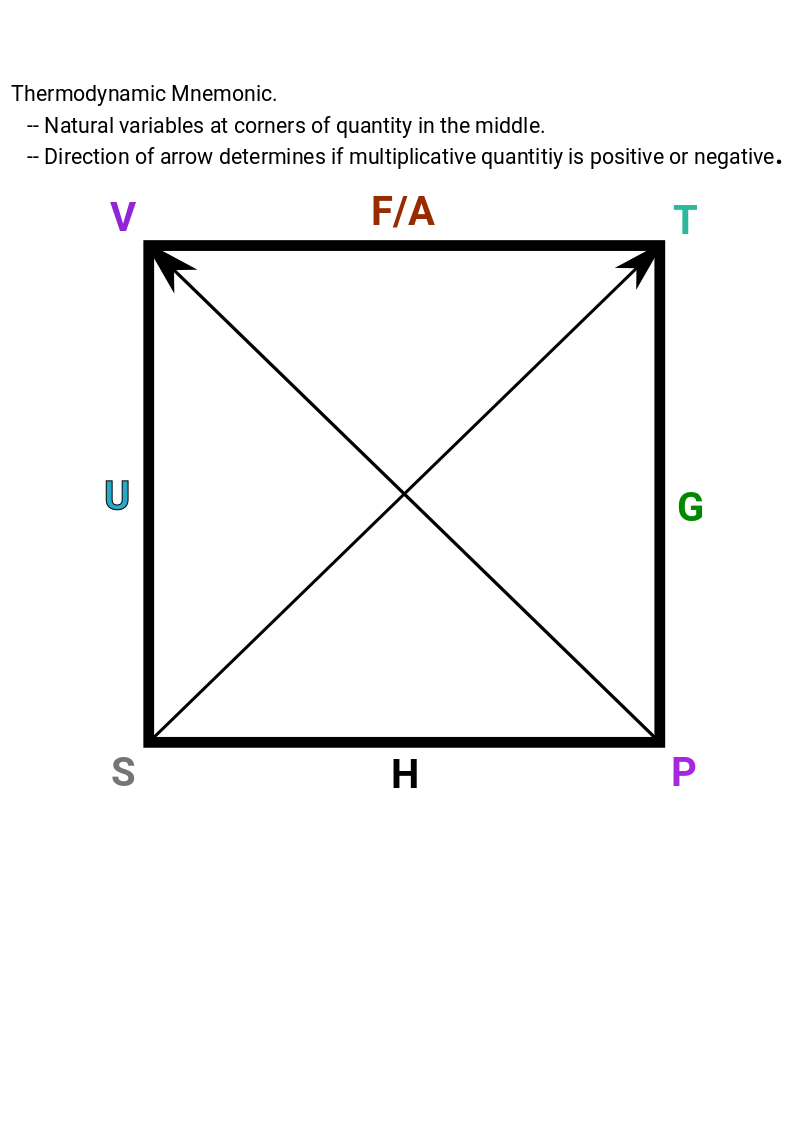
\includegraphics[width=.9\linewidth]{Images/Thermodynamic_mnemonic.png}
\end{center}


\section{Bibliography}
\label{sec:orge4dd1f1}
\label{org5217ed7}

\bibliographystyle{unsrt}
\bibliography{bibliography/org-refs}

\begin{LaTeX}
\bibliographystyle{unsrt}
\bibliography{./bibliiography/org-refs.bib}
\end{LaTeX}
\end{document}
